\section{Analysis Strategy and Event Selection}\label{sec:event_selection}
Two steps of analysis are taken. In the first step, a series of object and event selection was applied to maximize the sensitivity to detect the signal; in the second step,  a template fit on the 2-Dimension flavor weight distribution, which is got from TMVA based flavor tagging algorithm, is implemented to further distiguish the flavor components in final states. The details of template fit are described in \ref{sec:templatefit}.\par
The final states with 2 jets, 2 jets + 2 leptons(either electron or muon pair), 4 jets are required for \nnh,\llh and \qqh channel respectively.
\par
\subsection{$\llh$ Event Selection}
The $\llh$ channel is the composite of two sub-channels of $\eeh$ and $\mmh$ process. The dominant backgrounds are semi-leptonic $ZZ$ process and other $ZH$ production followed by other types of higgs decay(mainly by higgs decay to off-shell $W$ or $Z$ pair, and both intermediate boson undergo hadronic decay).
Two isolated tracks with opposite charge, reconstructed as electrons or muons, are required in addition to a pair of jets.  The recoil mass provide a very clear signature of the signal events, which have been delicately studied in \cite{CEPC:recoilmass}. 
The cut criteria of lepton pair recoil mass, together with the invariant mass of jet pair and lepton pair, are opptimized to maximum the signal significance. 
The polar angluar of the lepton pair recoil system are more concentrated in central region than the irreducible backgrounds from $t-$channel $ZZ$ production. The distribution of recoil and invariant masses and lepton pair
polar angluar distribution are presented in figure \ref{fig:kinematic_mumuh} and 
\ref{fig:kinematic_eeh} for $\mmh$ and $\eeh$ analysis.
To reject the background events from other higgs decay, y-value cut was set to suppress events with jet multiplicity other than 2. The signal and dominant backgrounds events yields after applying cuts are summarized in table \ref{tab:mumuh_cut} and \ref{tab:eeh_cut} for $\mmh$ and $\eeh$ analysis respectively.\par


\begin{figure}[!htpb]
\label{fig:kinematic_mumuh}
\centering
\subfigure[]
{
  \begin{minipage}[b]{0.42\textwidth}
  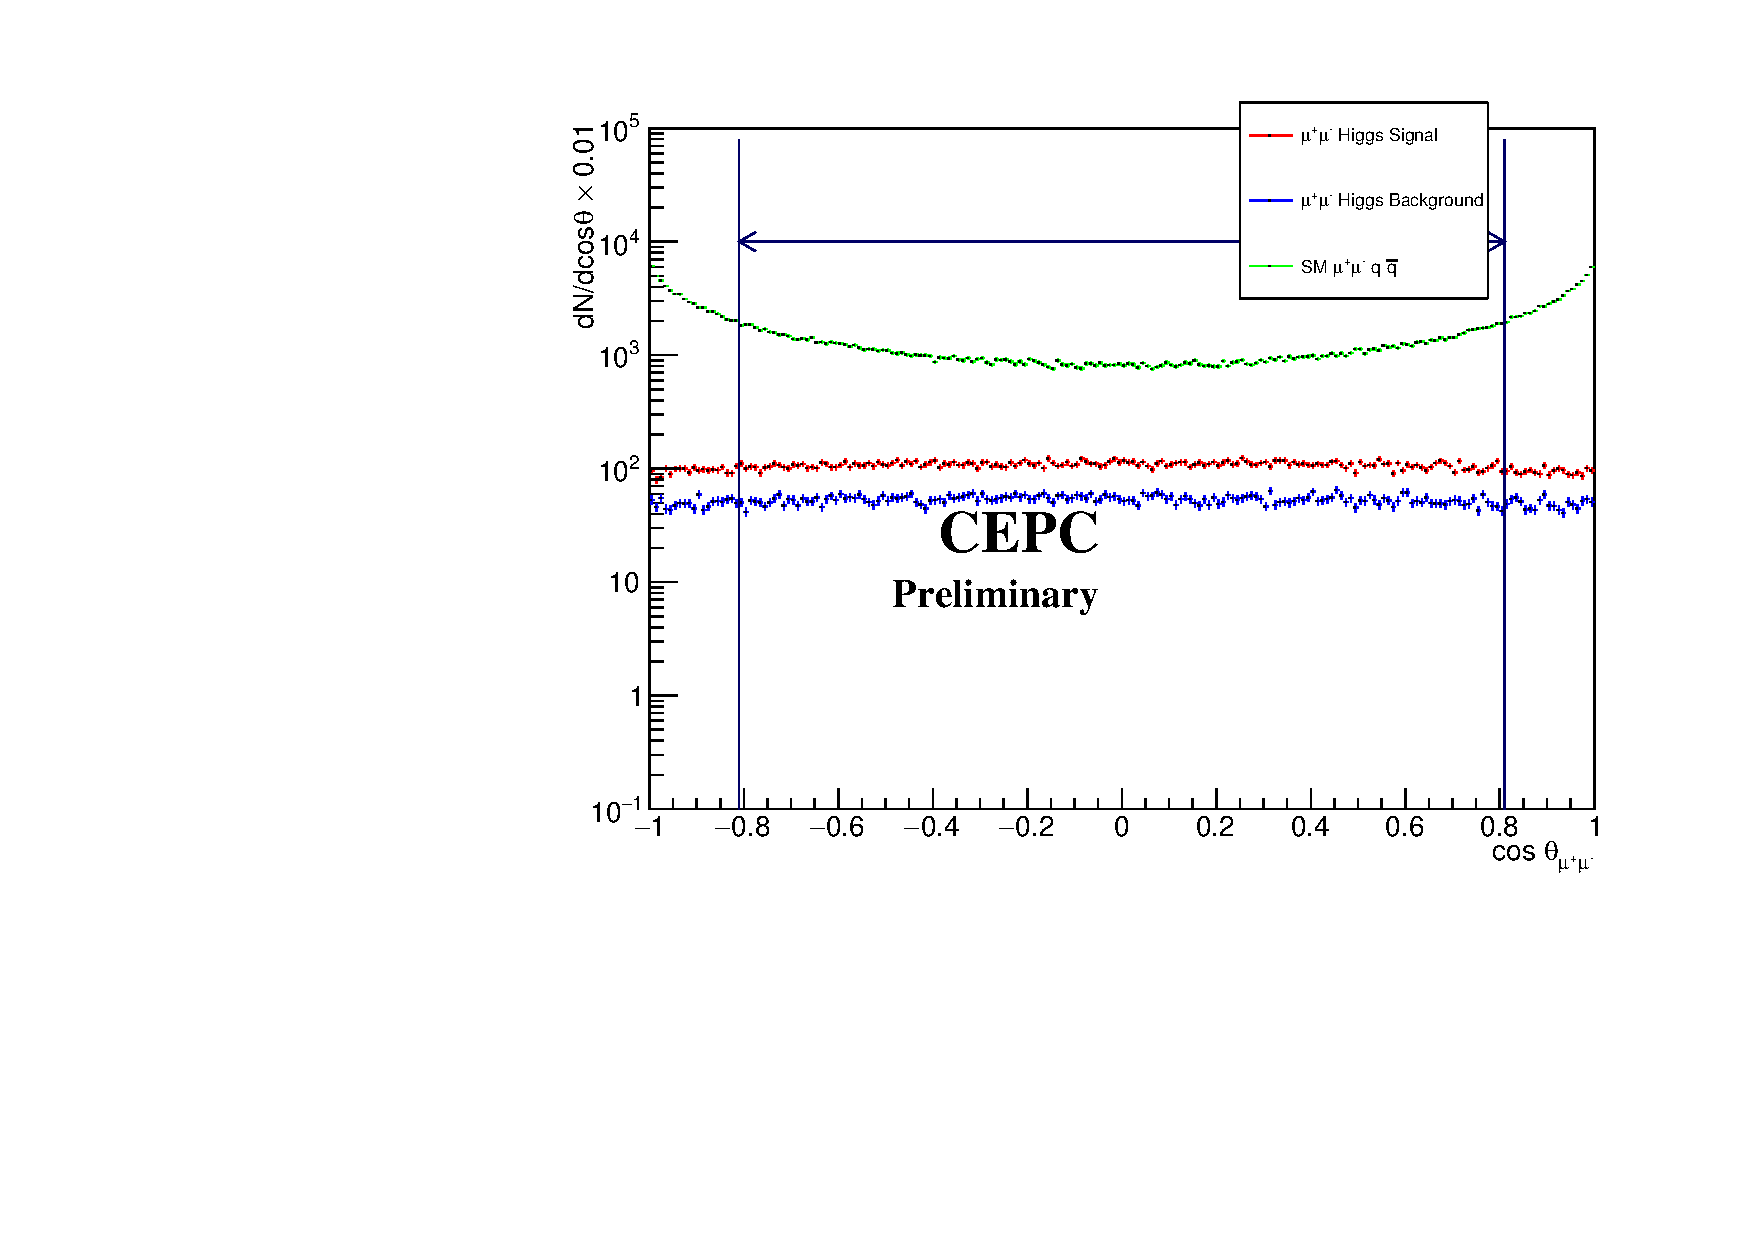
\includegraphics[width=\textwidth]{Analysis/mumuh/ZAngle.pdf}
  \end{minipage}
}
\subfigure[]
{
  \begin{minipage}[b]{0.42\textwidth}
  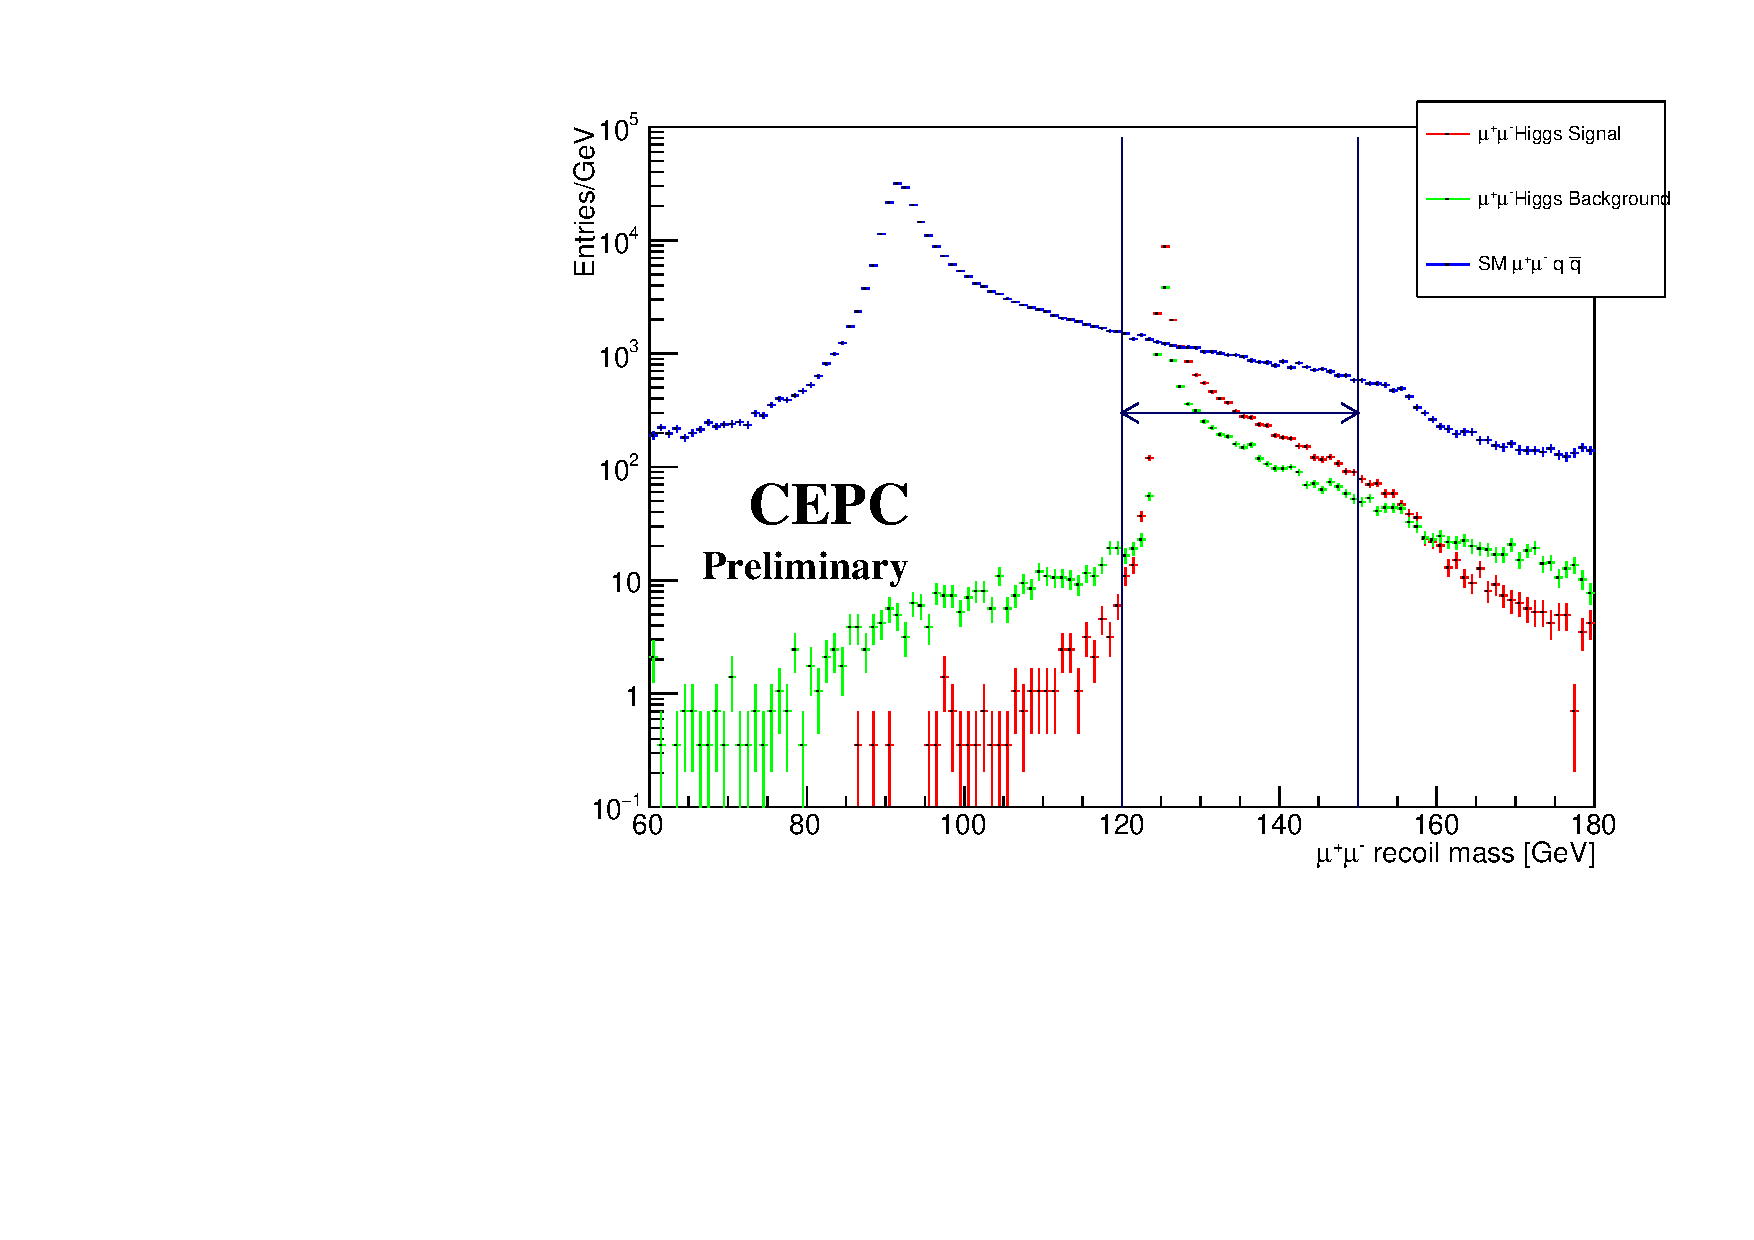
\includegraphics[width=\textwidth]{Analysis/mumuh/mumu_recoil.pdf}
  \end{minipage}
}
\subfigure[]
{ 
   \begin{minipage}[b]{0.42\textwidth}
   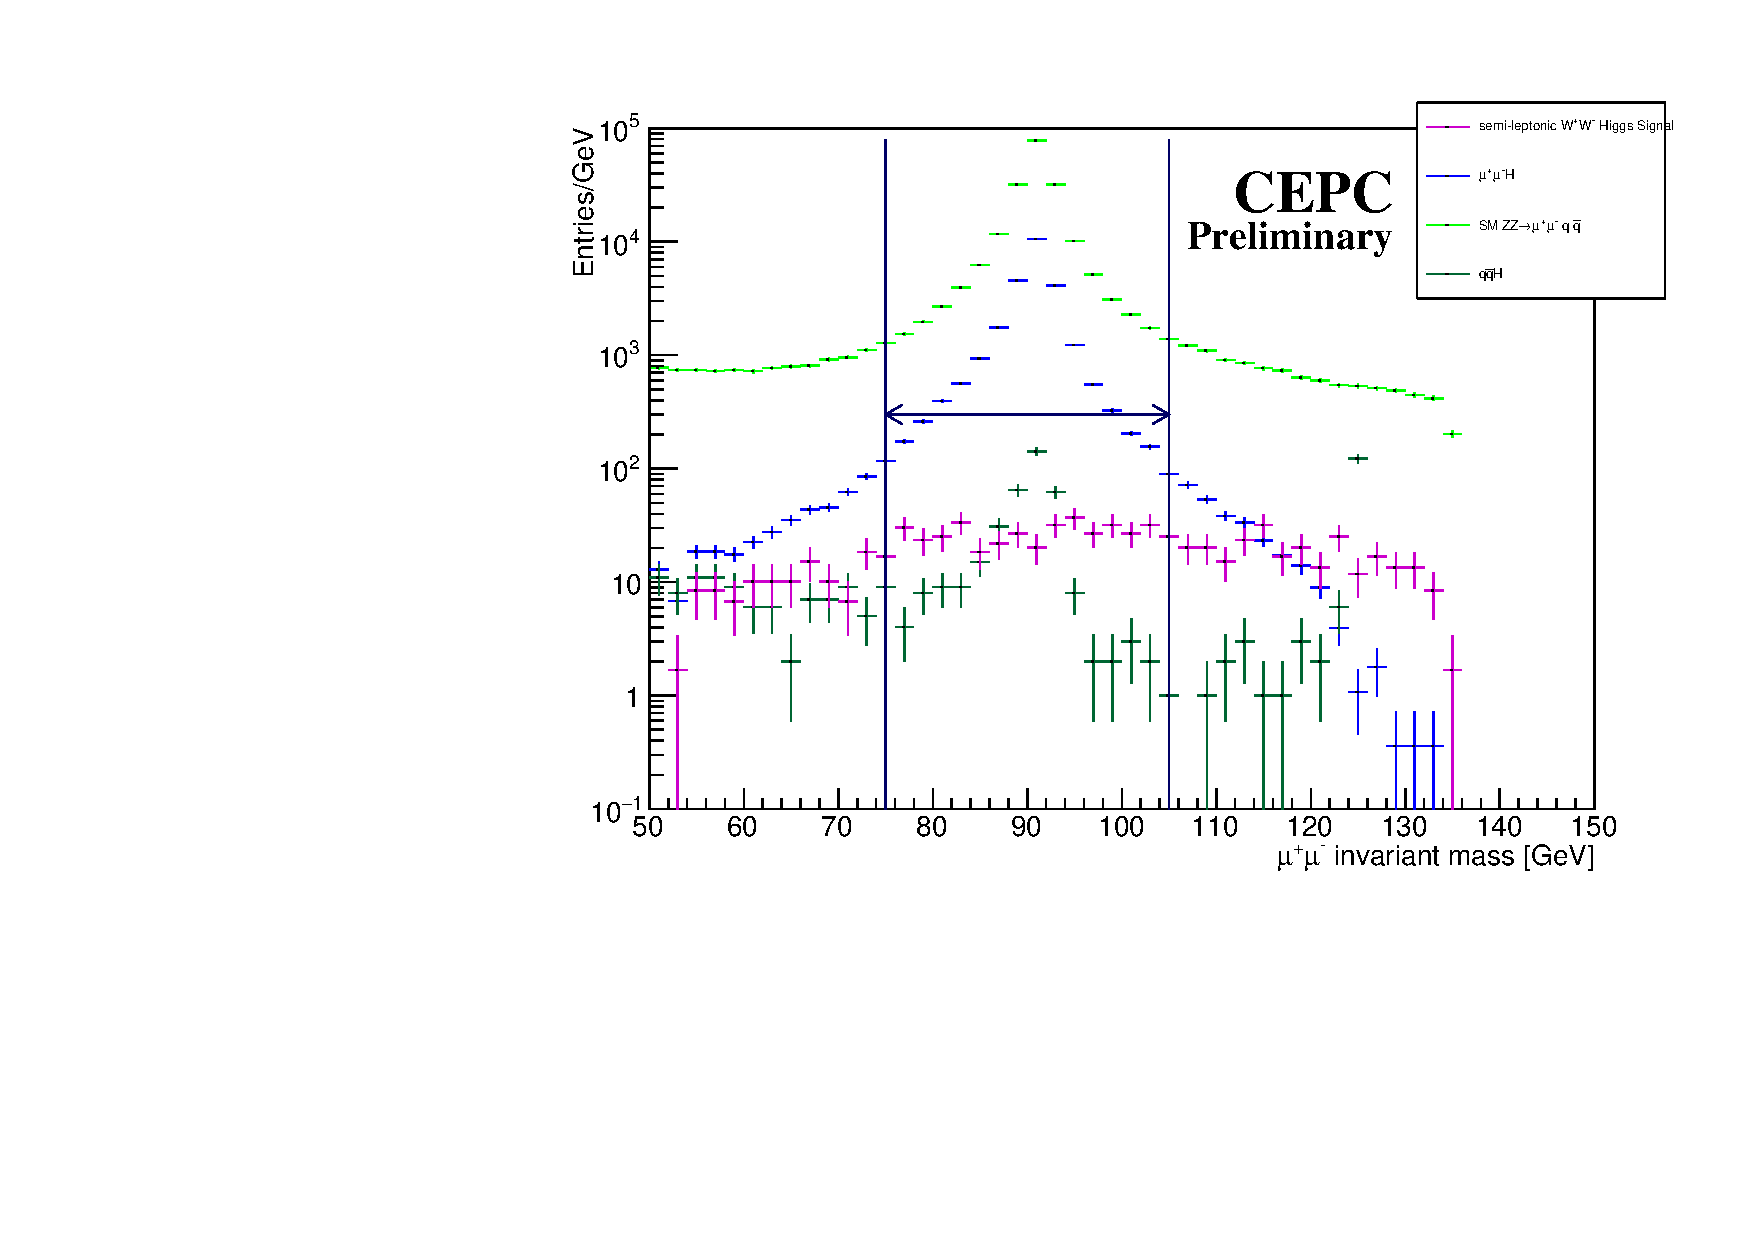
\includegraphics[width=\textwidth]{Analysis/mumuh/mumu_inv.pdf}
   \end{minipage}
}
\subfigure[]
{
    \begin{minipage}[b]{0.42\textwidth}
    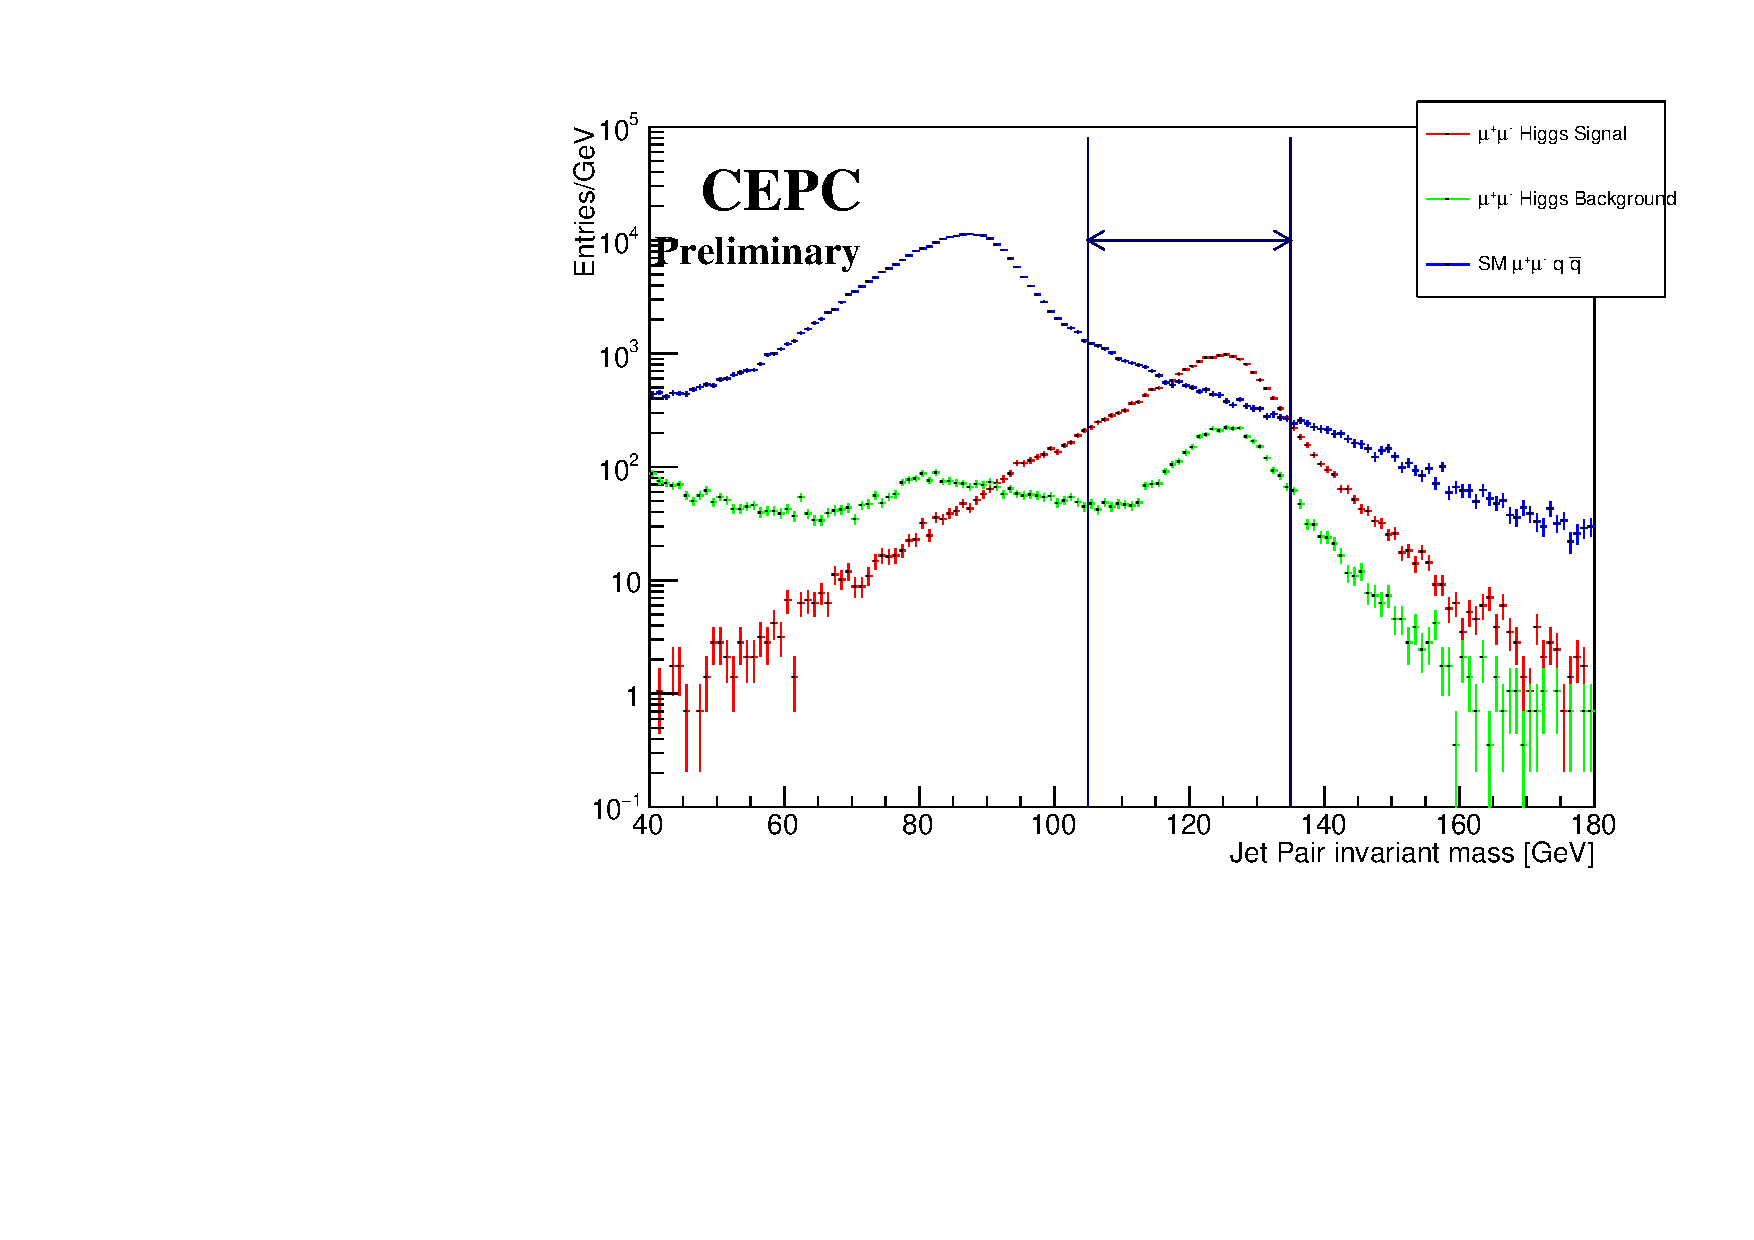
\includegraphics[width=\textwidth]{Analysis/mumuh/JJ_inv.pdf}
    \end{minipage}
}
\caption{Distribution of $\mu^+\mu^-$ system polar angle(top left), $\mu^+\mu^-$ recoil mass(top right), $\mu^+\mu^-$ invariant mass(bottom left) and jet pair invariant mass(bottom right) for signal and dominant backgrounds in $\mmh$ analysis.}
\end{figure}

\begin{table}[!htbp]
\label{tab:mumuh_cut}
\center
\begin{tabular}{c|c|c|c}\hline
%\multicolumn{4}{c|}{$\mmh$} \\ \hline
     Event Yields                          &     Signal   & $\mmh$ background  &  SM $\mu^+\mu^-q\bar{q}$ process \\ \hline
     $\sigma\times$Lumi                    &     24532.3  &      10967.6    &     1051700\\ \hline
       Object Selection                    &     17563.7  &      9203.5                     &    296779.5        \\ \hline
0.85$<\cos\theta_{\mu^+\mu^-}<$0.85        &     18580.8 &      8213.7                         &    193043.4
\\ \hline
120 \GeV$<M_{\mu^+\mu^-recoil}<$150 \GeV   &     17953.2  &      7849.6                       &     19711.2 
\\ \hline 
70 \GeV$<M_{\mu^+\mu^-}<$105               &     17557.1  &      7255.4
&17485.2  \\ \hline
105 \GeV$<M_{JJ}<$135 \GeV                 &     14392.6  &      2927.0 
& 5769.2   \\ \hline
$y_{23}$ \& $y_{34}$ cut                   &     13707.8  &      1575.2 
& 5152.8   \\ \hline 
\end{tabular}
\caption{Event Yields of signal and dominant backgrounds with cuts of $\mmh$ channel, normalized to 5000 \ifb.}
\end{table}

\begin{figure}[!htbp]
\label{fig:kinematic_eeh}
\centering
\subfigure[]
{
  \begin{minipage}[b]{0.42\textwidth}
  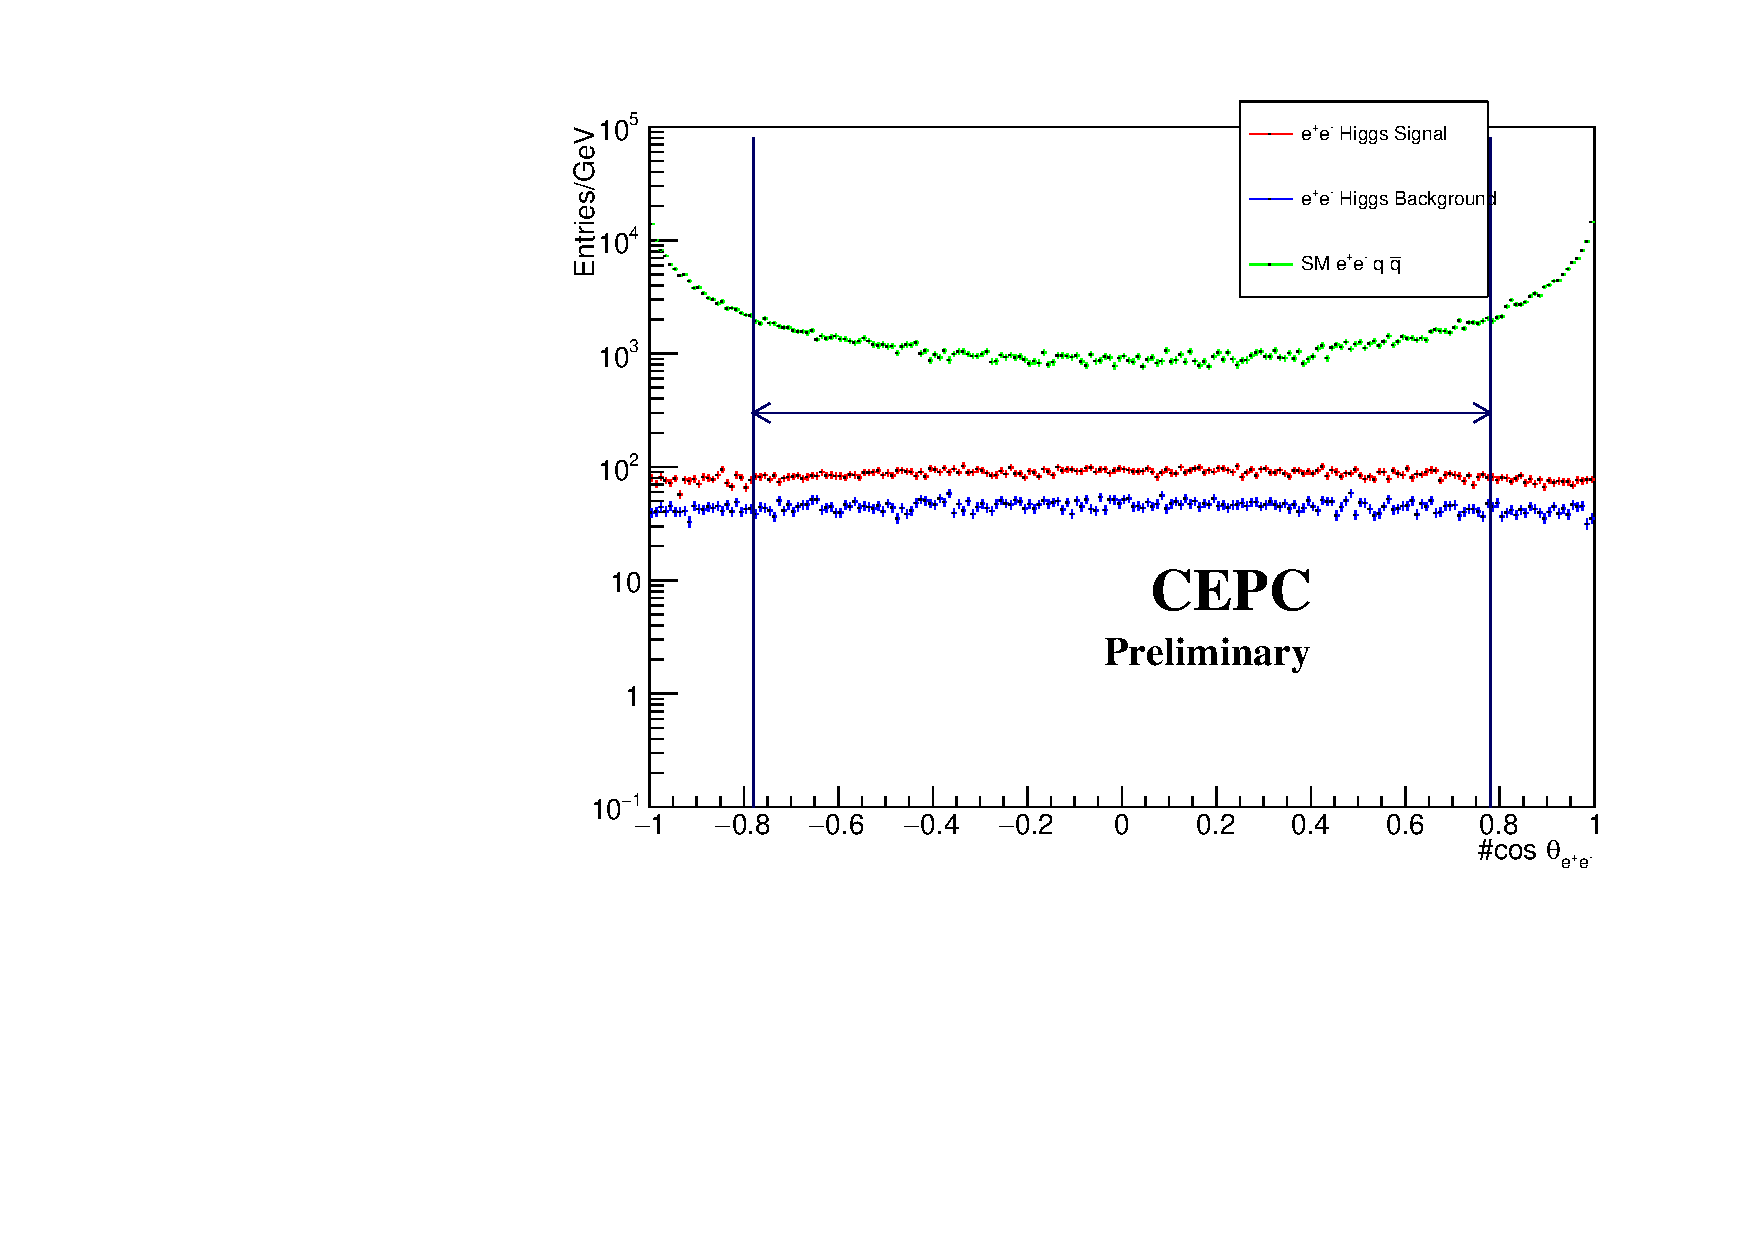
\includegraphics[width=\textwidth]{Analysis/eeh/ZAngle_ee.pdf}
  \end{minipage}
}
\subfigure[]
{
  \begin{minipage}[b]{0.42\textwidth}
  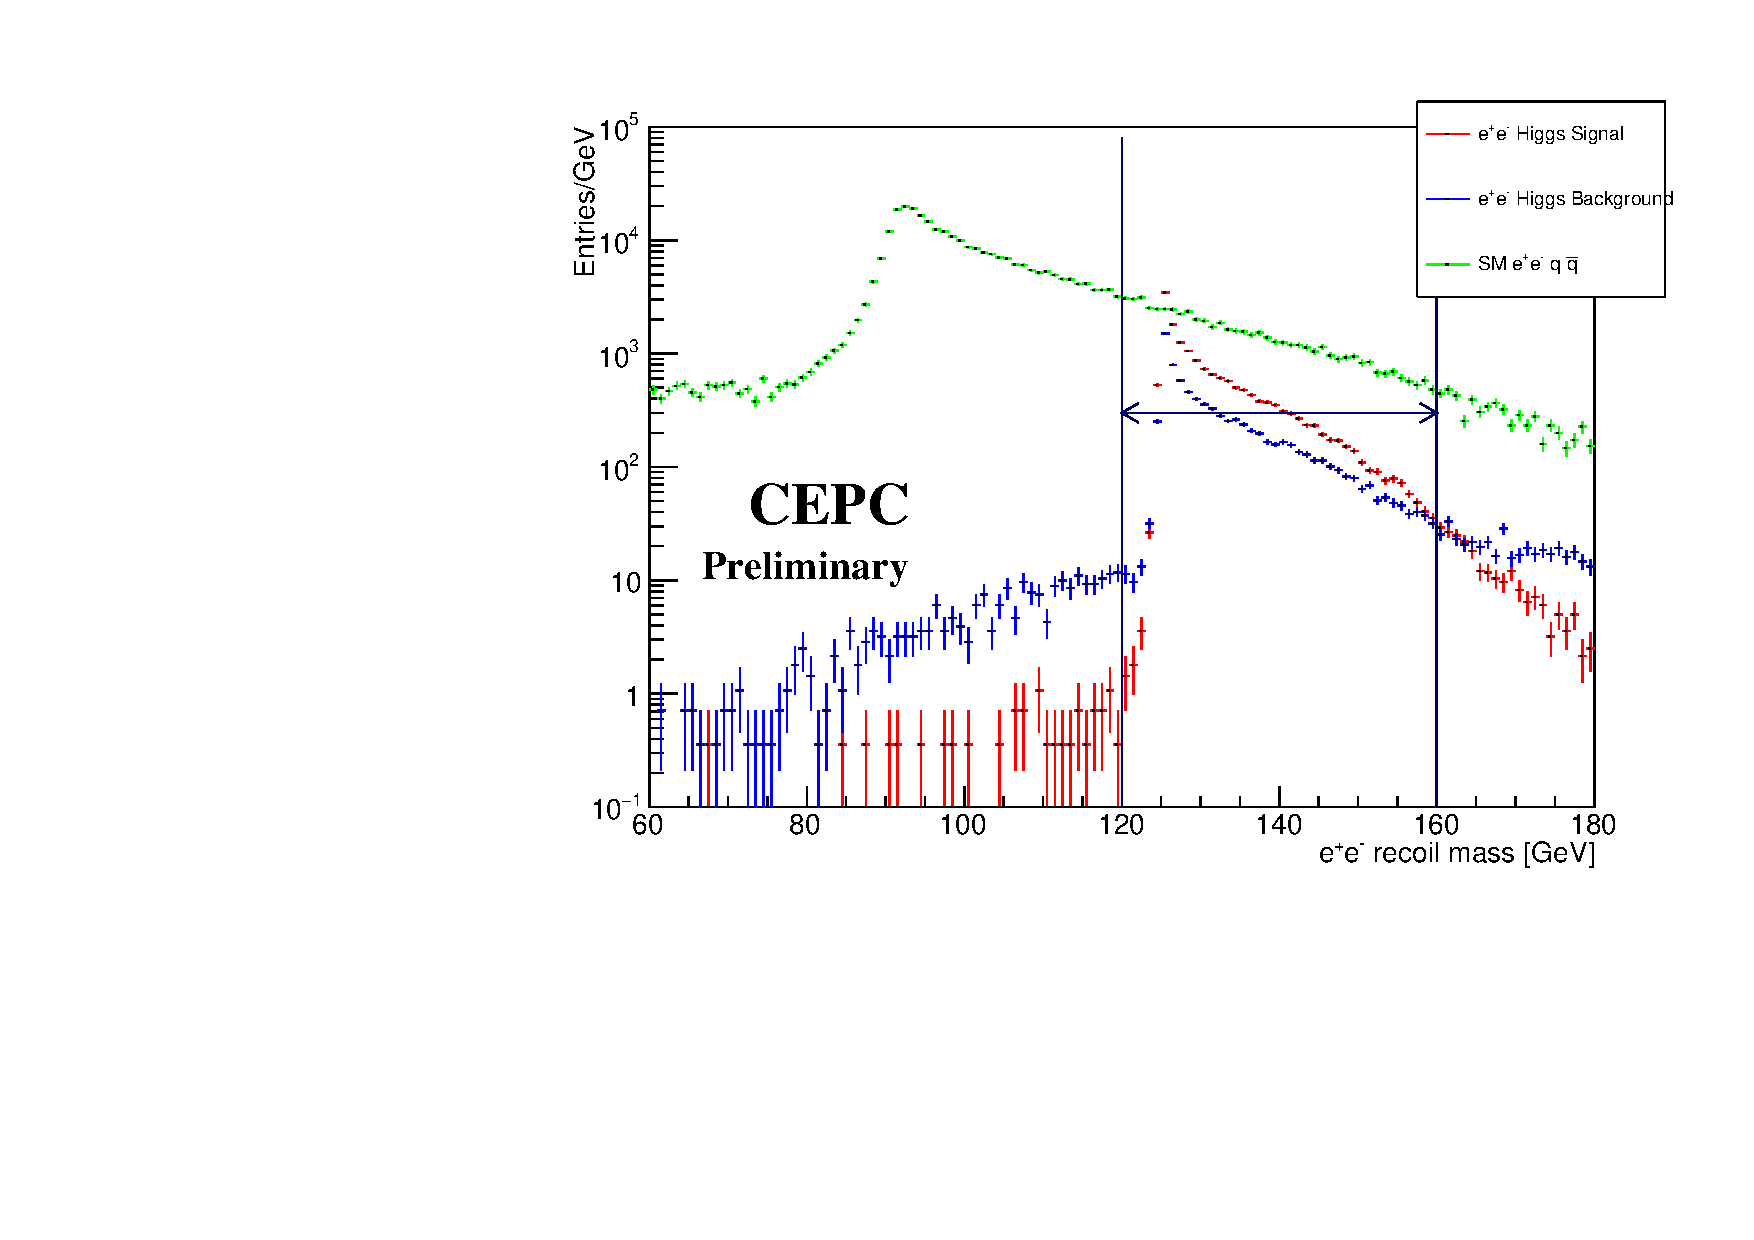
\includegraphics[width=\textwidth]{Analysis/eeh/ee_recoil.pdf}
  \end{minipage}
}
\subfigure[]
{ 
   \begin{minipage}[b]{0.42\textwidth}
   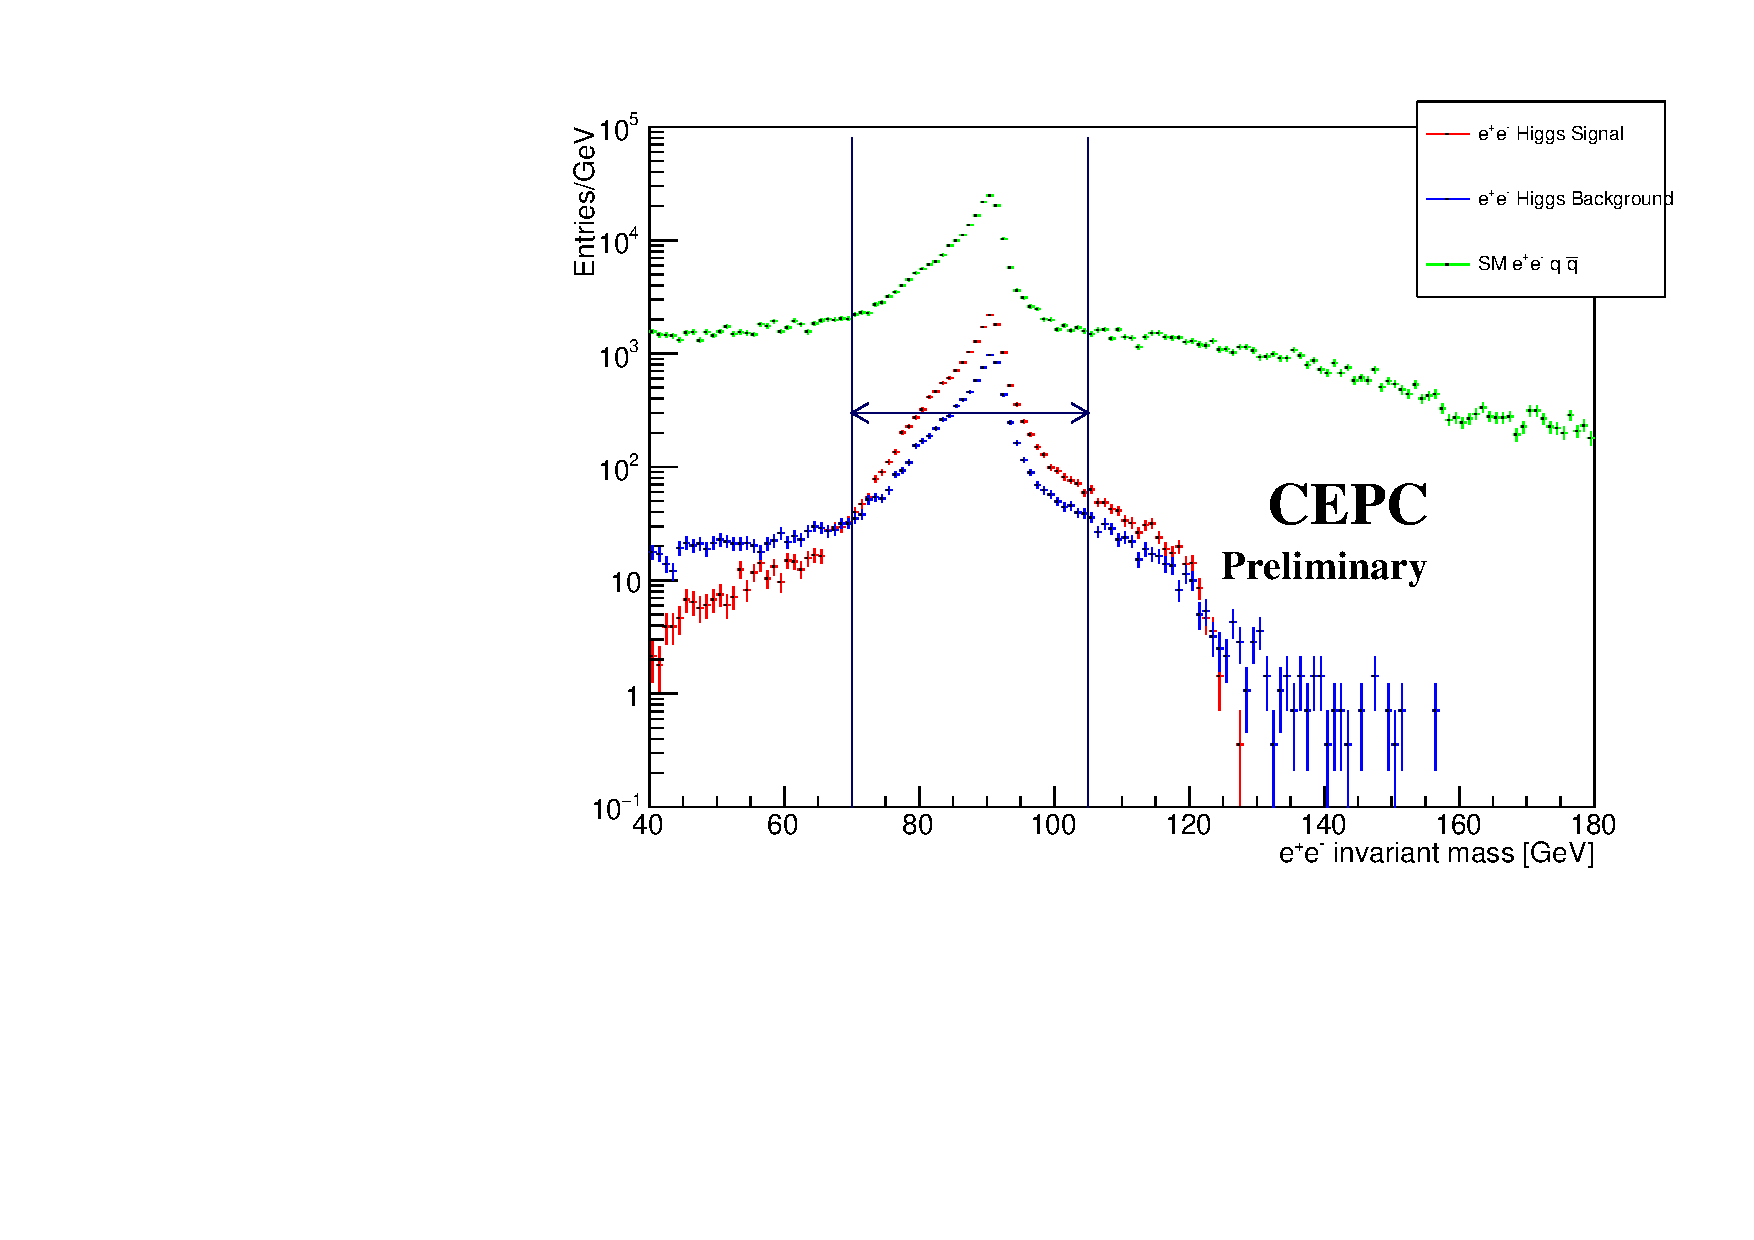
\includegraphics[width=\textwidth]{Analysis/eeh/ee_inv.pdf}
   \end{minipage}
}
\subfigure[]
{
    \begin{minipage}[b]{0.42\textwidth}
    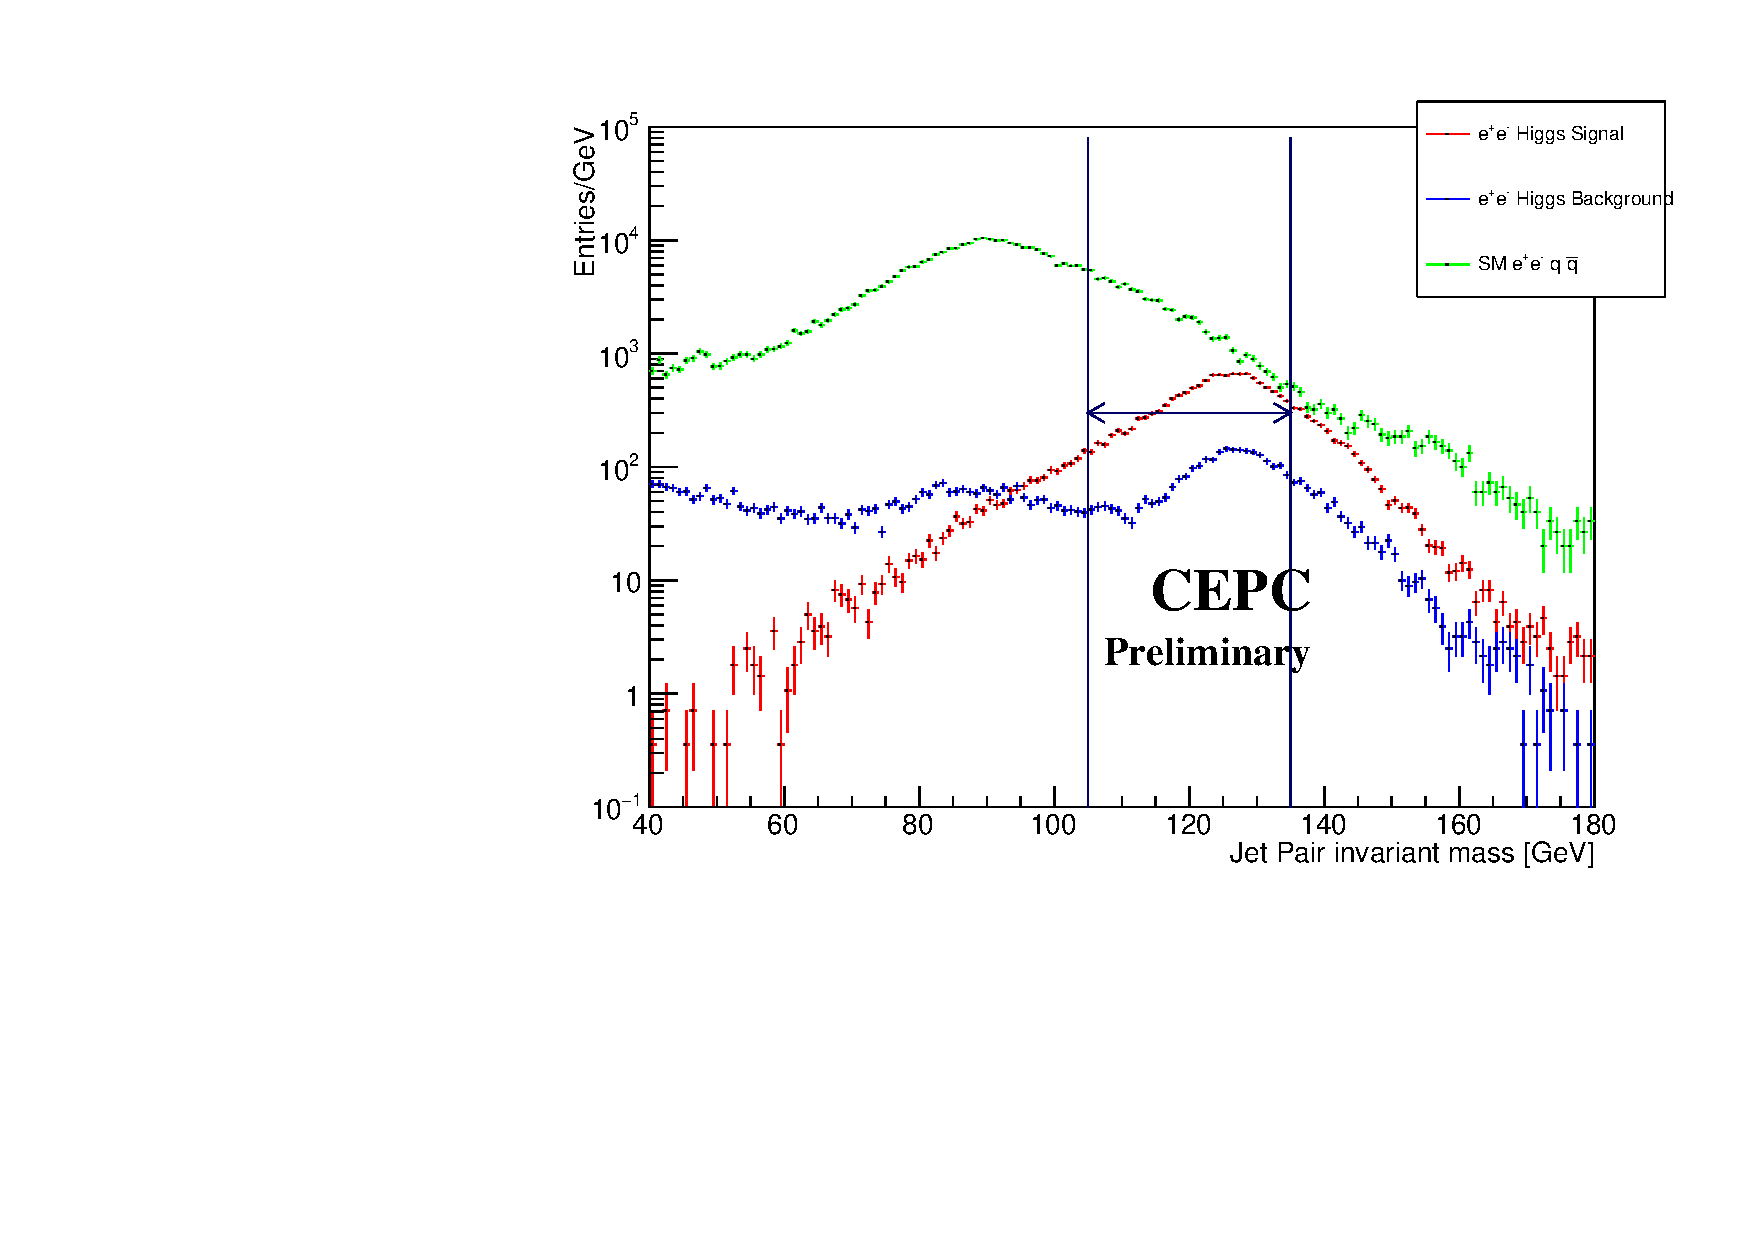
\includegraphics[width=\textwidth]{Analysis/eeh/jj_inv_ee.pdf}
    \end{minipage}
}
\caption{Distribution of $e^+e^-$ system polar angle(top left), $e^+e^-$ recoil mass(top right), $e^+e^-$ invariant mass(bottom left) and jet pair invariant mass(bottom right) for signal and dominant backgrounds in $\eeh$ analysis.}
\end{figure}

\begin{table}[!htbp]
\label{tab:eeh_cut}
\center
\begin{tabular}{c|c|c|c}\hline
%\multicolumn{4}{c|}{$\mmh$} \\ \hline
     Event Yields                          &     Signal   & $\eeh$ background  &  SM $e^+e^-q\bar{q}$ process \\ \hline
     $\sigma\times$Lumi                    &     26438.4  &     11918.6 &   1639129  \\ \hline
       Object Selection                    &     21245.7  &      9192.0                     &    296779.5        \\ \hline
0.78$<\cos\theta_{e^+e^-}<$0.78        &     14002.0  &      7200.8                         &    372942.9
\\ \hline
120 \GeV$<M_{e^+e^-recoil}<$160 \GeV   &     13773.9  &      6581.0                         &    167607.0 
\\ \hline 
70 \GeV$<M_{e^+e^-}<$105               &     13143.0  &      6051.4
&27027.4  \\ \hline
105 \GeV$<M_{JJ}<$135 \GeV                 &     9637.7   &      1935.3 
& 6941.2   \\ \hline
$y_{23}$ \& $y_{34}$ cut                    &    9148.4  &       1101.9 
& 6081.4   \\ \hline 
\end{tabular}
\caption{Event Yields of signal and dominant backgrounds with cuts of $\eeh$ channel, normalized to 5000 \ifb.}
\end{table}
%\clearpage

\subsection{\nnh Event Selection}
The \nnh channel includes $ZH$ production followed by invisible $Z-$decay, or $t-$channel $W-$fusion process. 
The dominant backgrounds are quark pair production and gauge boson pair production, followed by hadronic and invisible decay of each boson. 
The observable particles in the signal form two energetic jets, initiated from two quarks of higgs decay. 
Thus isolation leptons are rejected, and a minimum number of PFOs are required the quark pair. 
The signal events are featured in the kinematic distribution of invisible section.  
The visible energy of the signal events are significantly lower than reducible SM backgrounds like semi-leptonic $WW$ events. 
The visible transverse momentum are required to larger than 19 \GeV to reject \qq events, which tend to have low visible tranverse momentum due to 
high fraction of radiation return events.
The invariant mass of the jets characterize the higgs production which is obverse discriminator against the non-higgs production SM events
\footnote{The peak of in signal region of \qq events is due to radiation events.}.
The angle between two jets and $y$-th values are also useful to distinguish signal events from SM backgrounds.  
Meanwhile the recoil system of these two jets, which is not directly observable, has the charaterstic of the $Z$ boson associate with higgs in final states. The distribution of the above varibles and cut value can be found in figure \ref{fig:kinematic_nnh} and \ref{fig:yth_nnh} for signal and background events. \par

The Boost decision tree \cite{BDT} method is implemented to the survived events from cut chain. The variables used 
in BDT are mentioned aboved: visible energy,  transverse momentum, $y-th$ value, jet pair recoil and invariant mass. 
The events yields of signal and background in cutflow and BDT selection can be found in table \ref{tab:nnh_cut}. \par


\begin{figure}[!htbp]
\label{fig:kinematic_nnh}
\centering
\subfigure[]
{
  \begin{minipage}[b]{0.31\textwidth}
  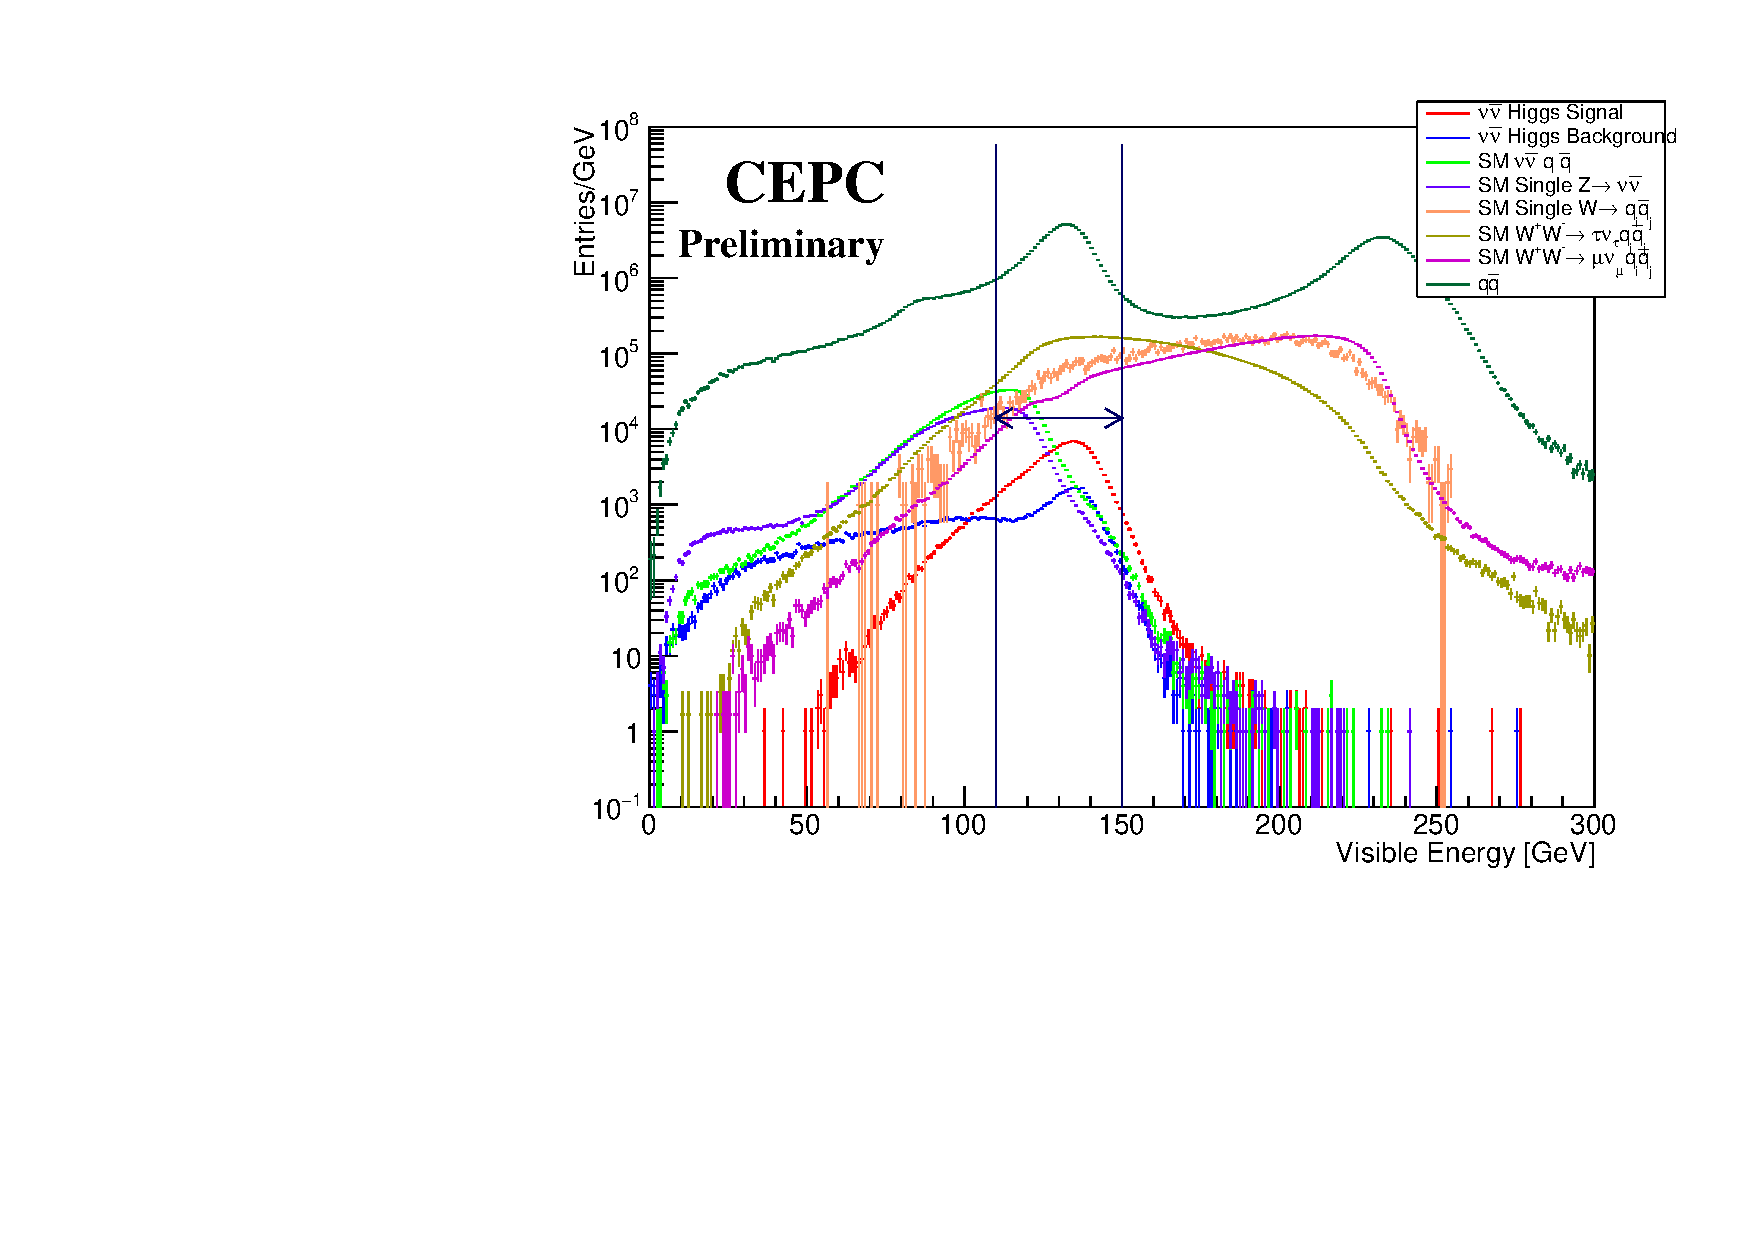
\includegraphics[width=\textwidth]{Analysis/nnh/Etot.pdf}
  \end{minipage}
}
\subfigure[]
{
  \begin{minipage}[b]{0.31\textwidth}
  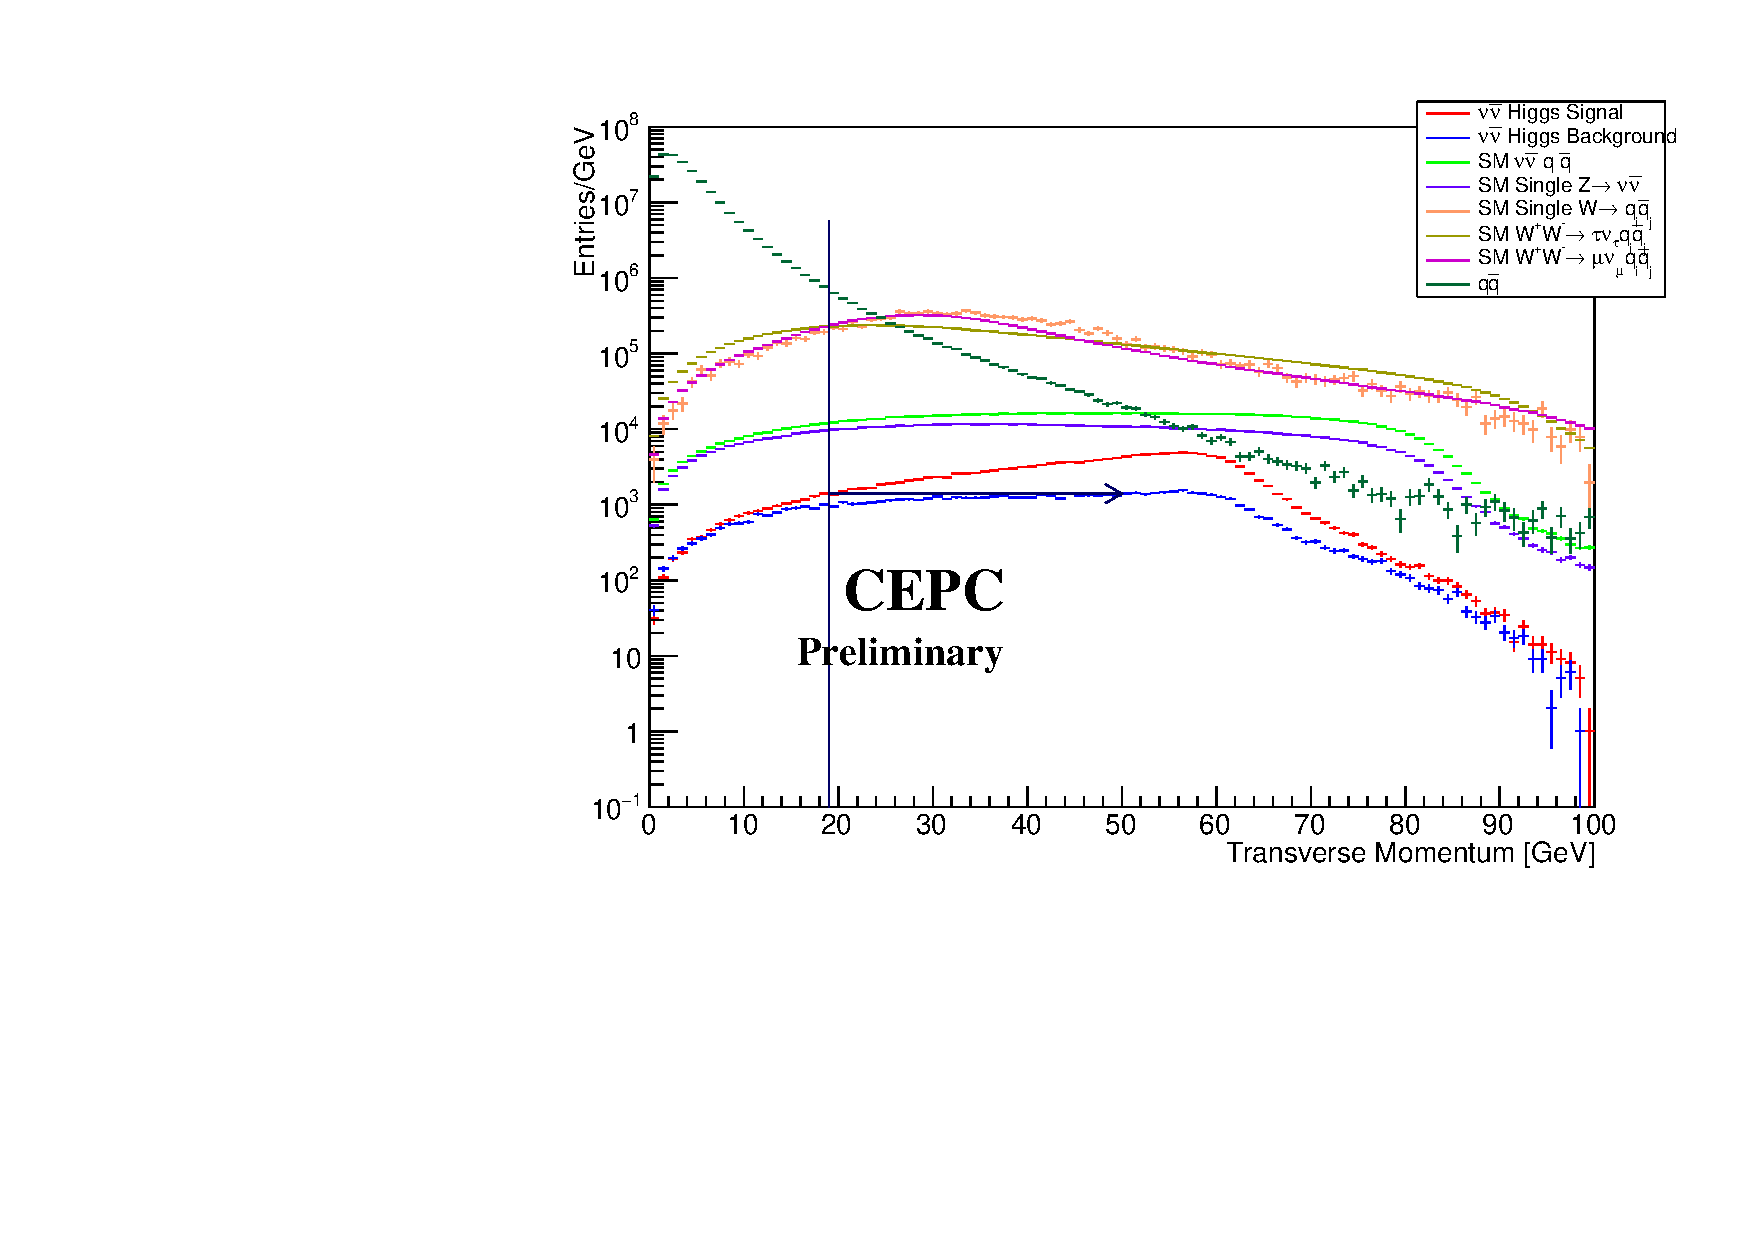
\includegraphics[width=\textwidth]{Analysis/nnh/pT.pdf}
  \end{minipage}
}
\subfigure[]
{
  \begin{minipage}[b]{0.31\textwidth}
  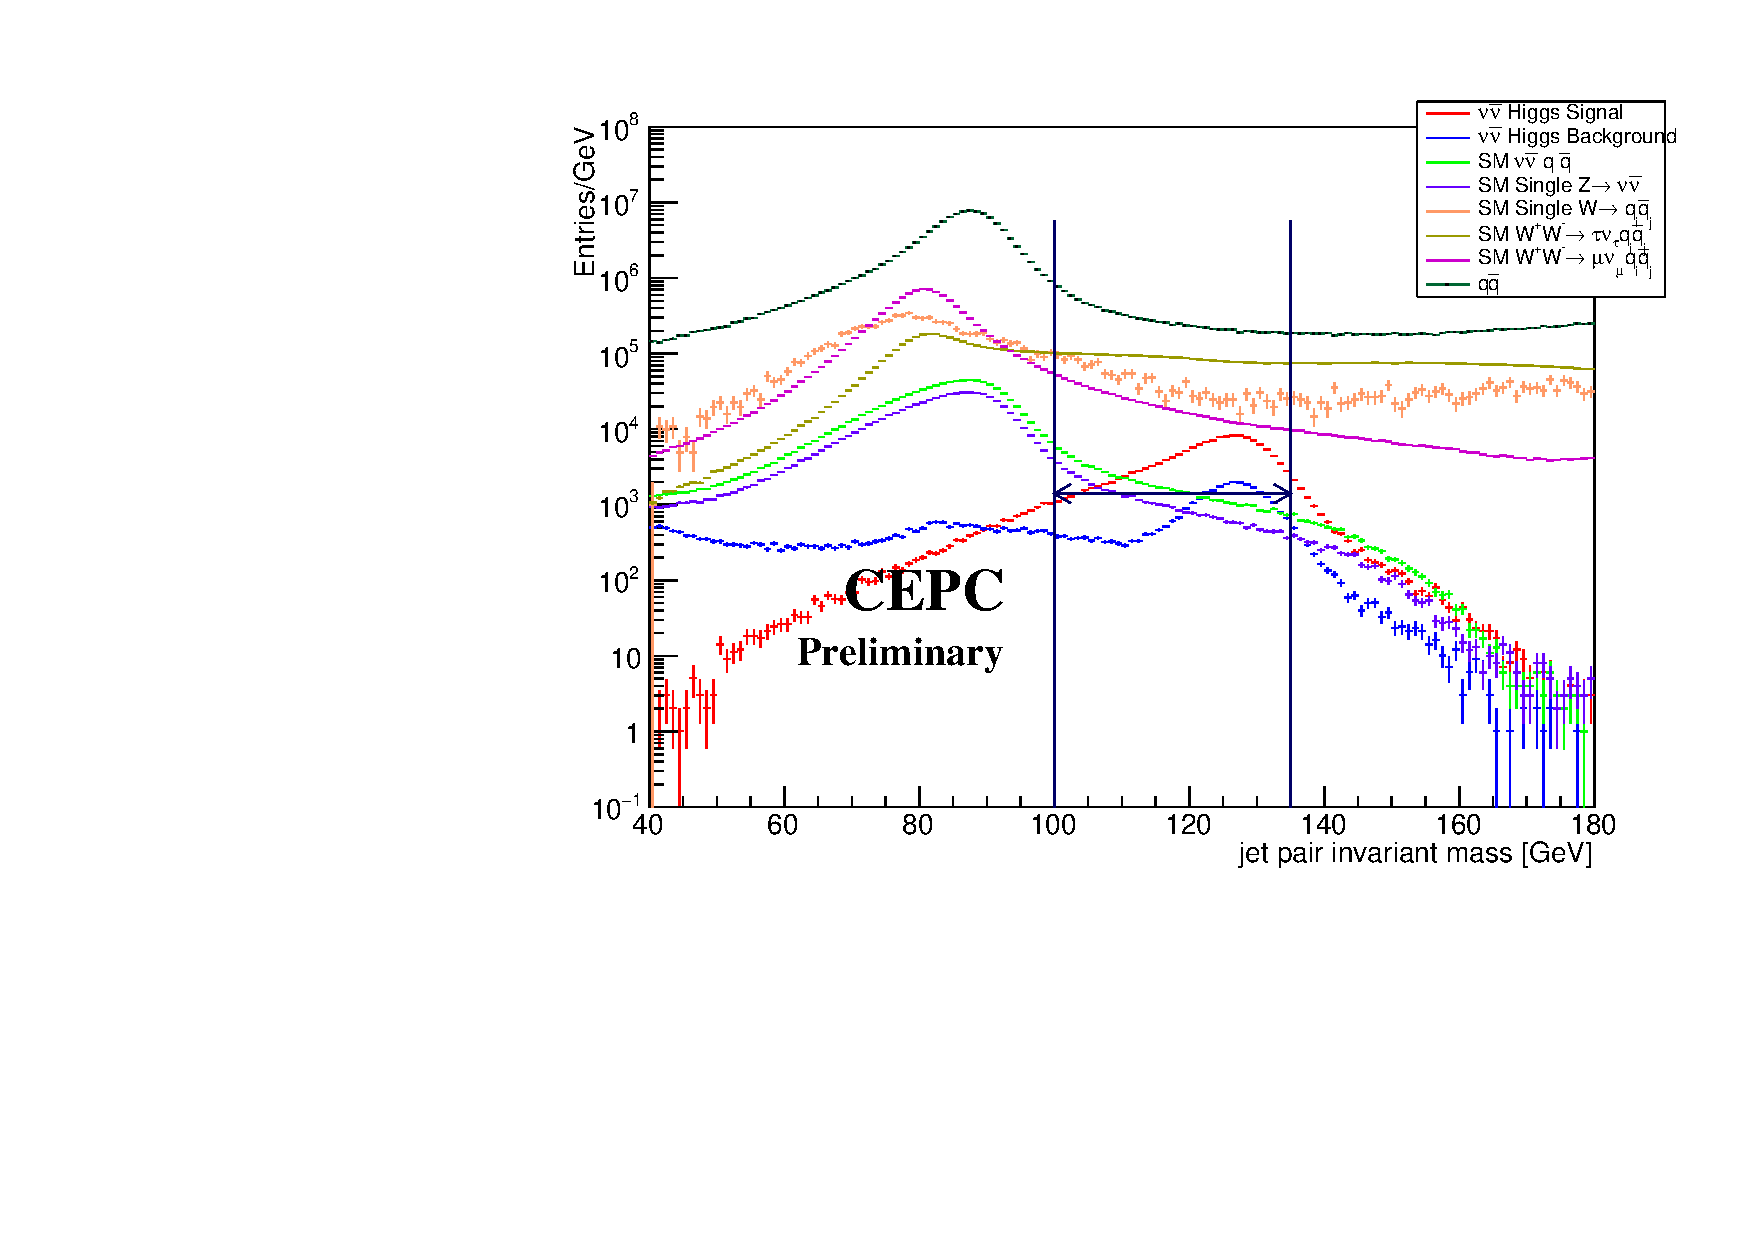
\includegraphics[width=\textwidth]{Analysis/nnh/jj_inv.pdf}
  \end{minipage}
}
\subfigure[]
{ 
   \begin{minipage}[b]{0.31\textwidth}
   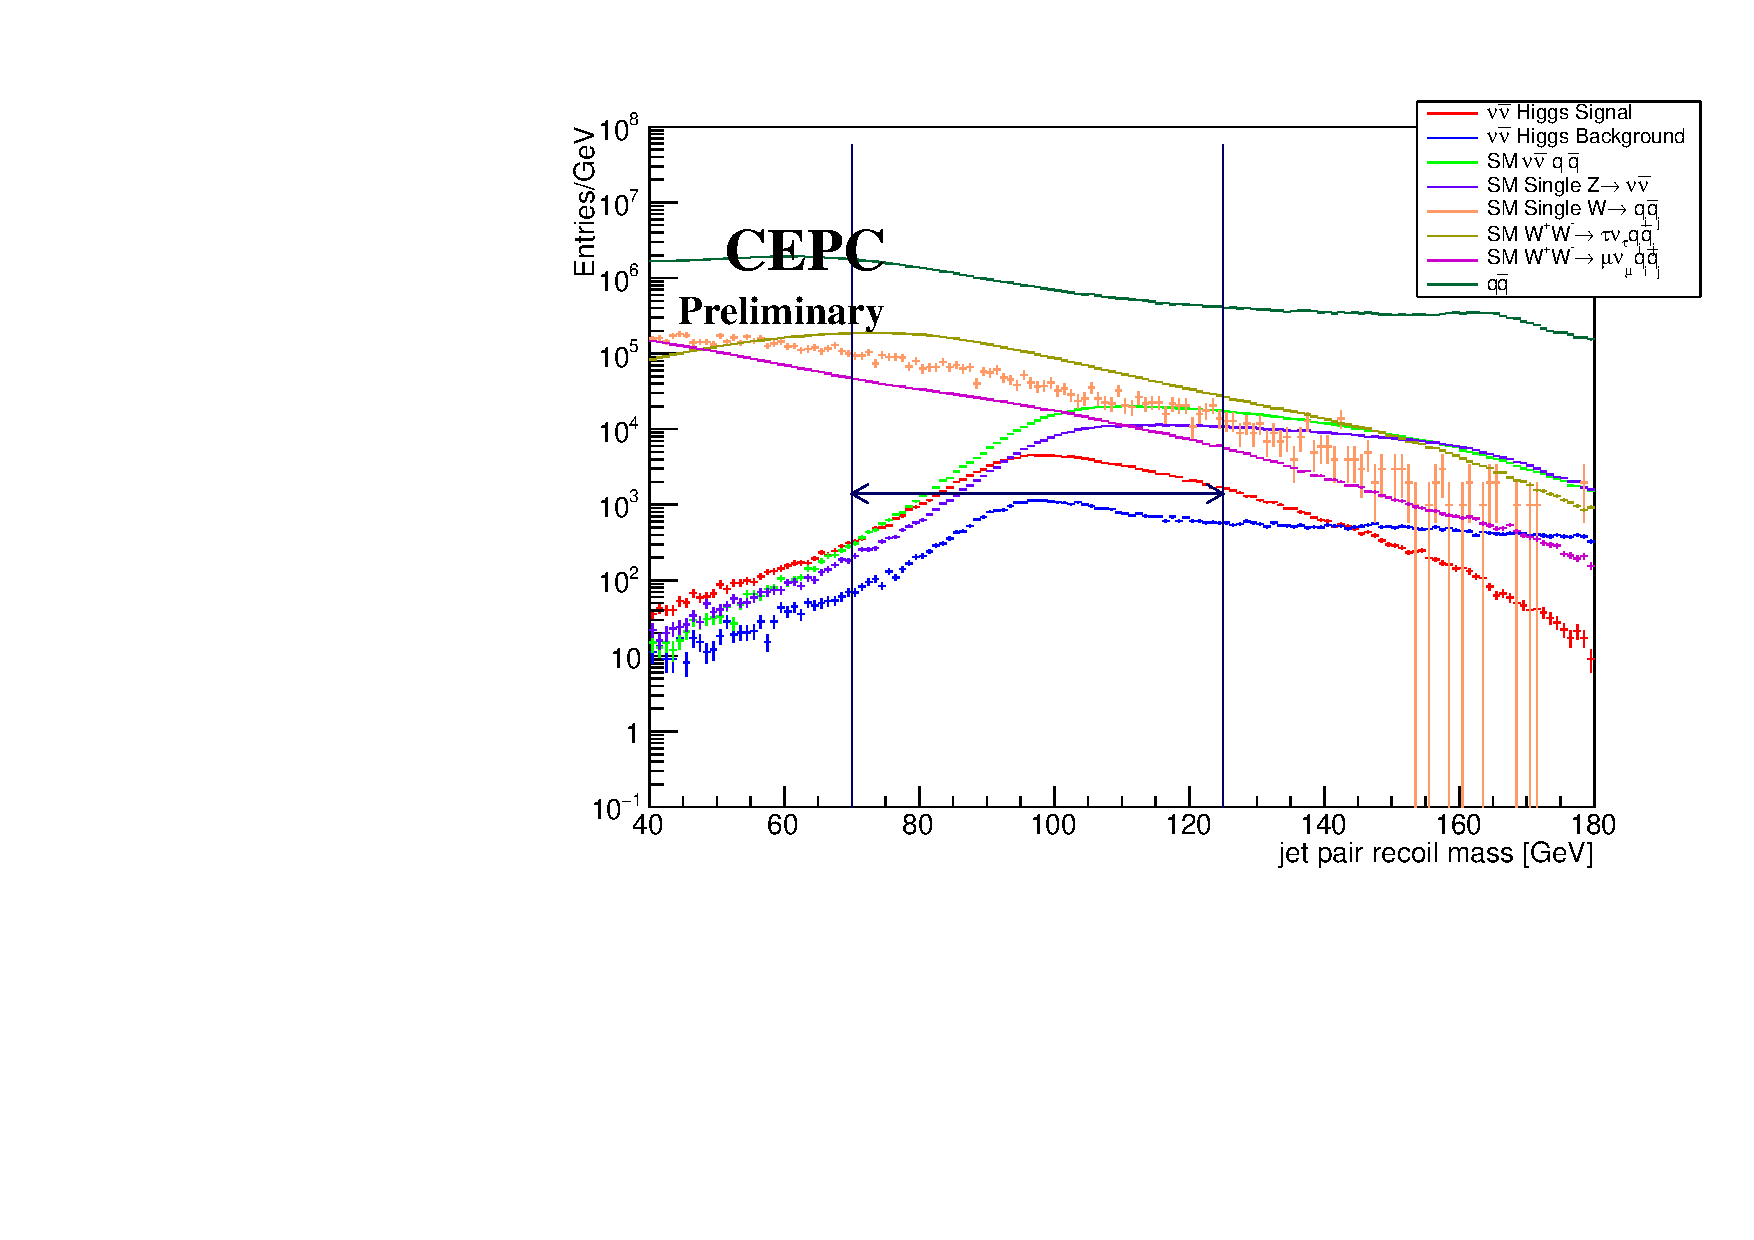
\includegraphics[width=\textwidth]{Analysis/nnh/jj_recoil.pdf}
   \end{minipage}
}
\subfigure[]
{
    \begin{minipage}[b]{0.31\textwidth}
    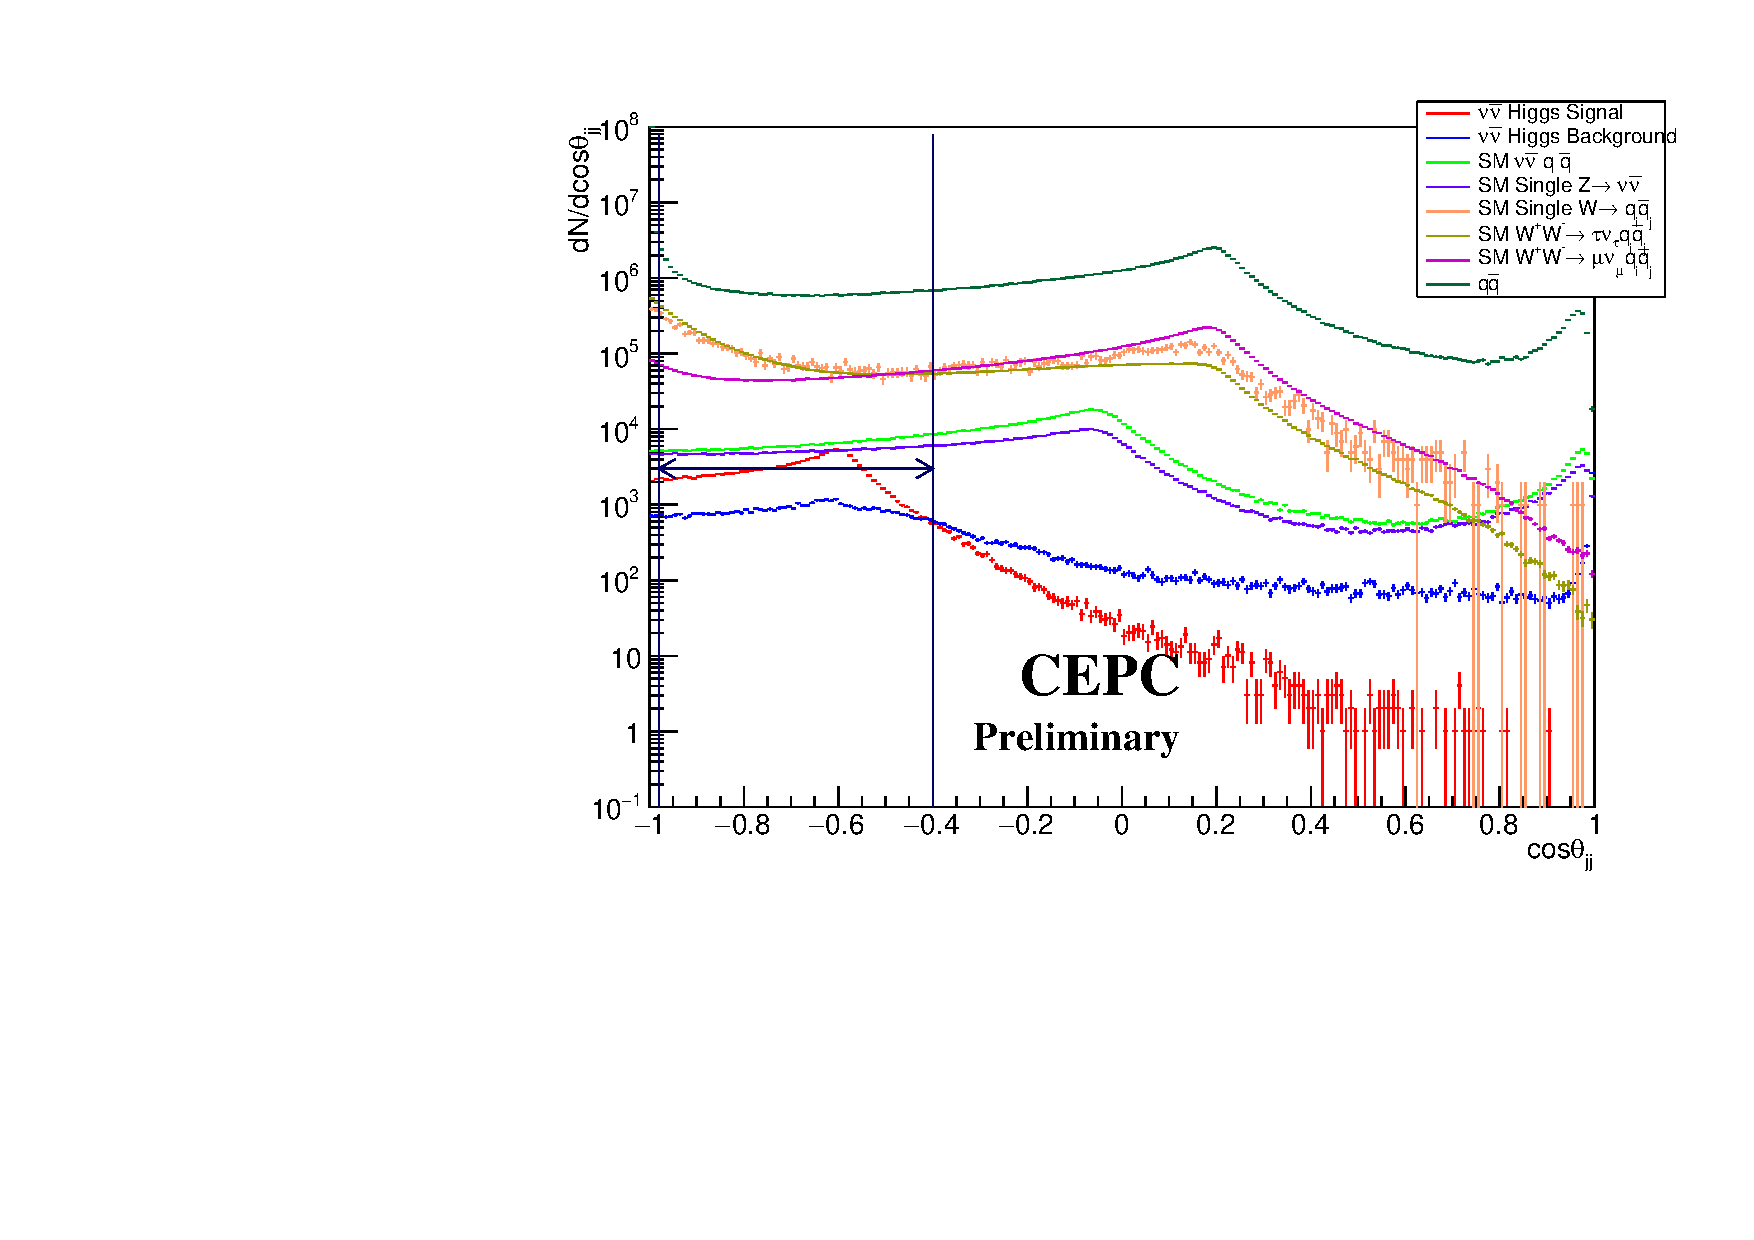
\includegraphics[width=\textwidth]{Analysis/nnh/costheta.pdf}
    \end{minipage}
}
\caption{Visible energy(top left), visible transverse momentum(top middle), jet pair system invariant mass(top right), jet system recoil mass(bottom left) and jet pair system polar angluar(bottom right) distribution in \nnh analysis.}
\end{figure}

\begin{figure}[!htpb]
\label{fig:yth_nnh}
\centering
\subfigure[]
{
  \begin{minipage}[b]{0.31\textwidth}
  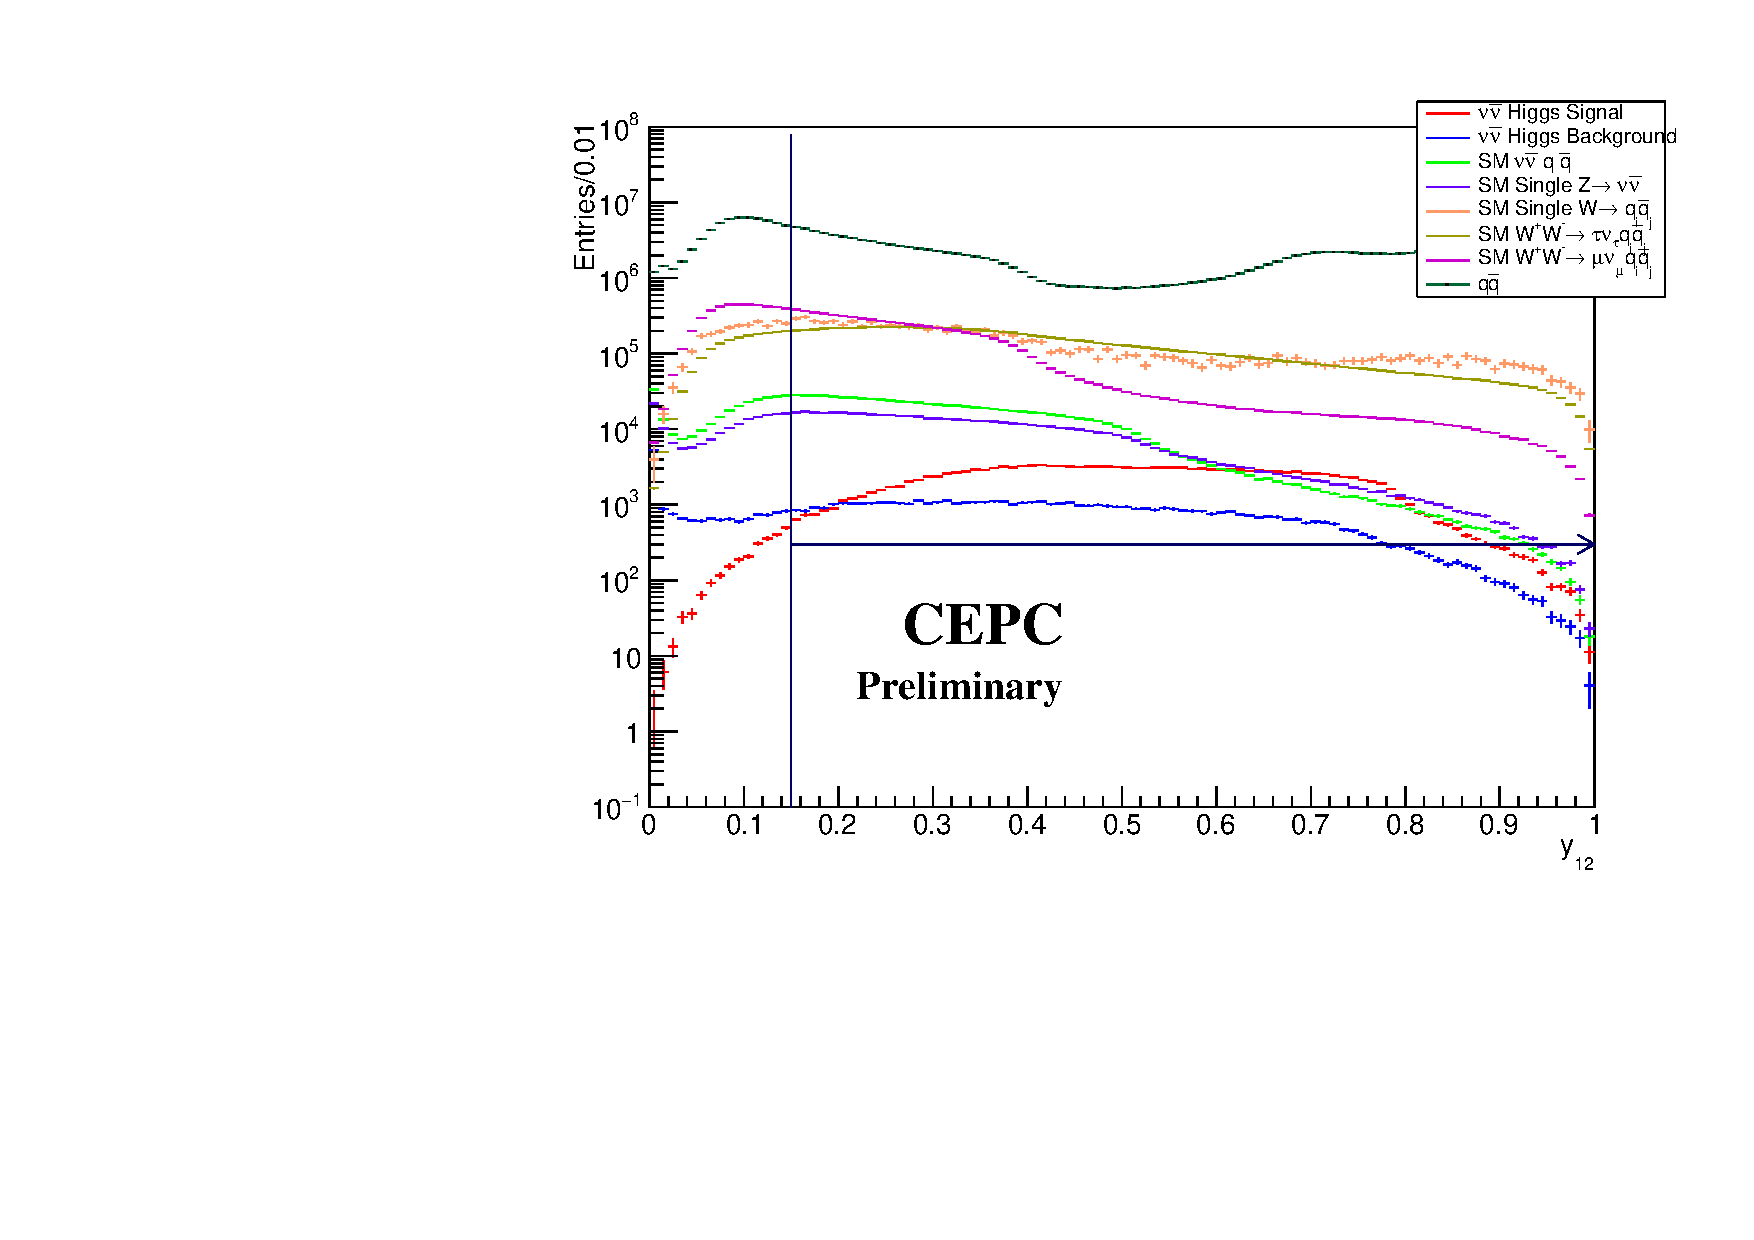
\includegraphics[width=\textwidth]{Analysis/nnh/y12.pdf}
  \end{minipage}   
}
\subfigure[]
{
  \begin{minipage}[b]{0.31\textwidth}
  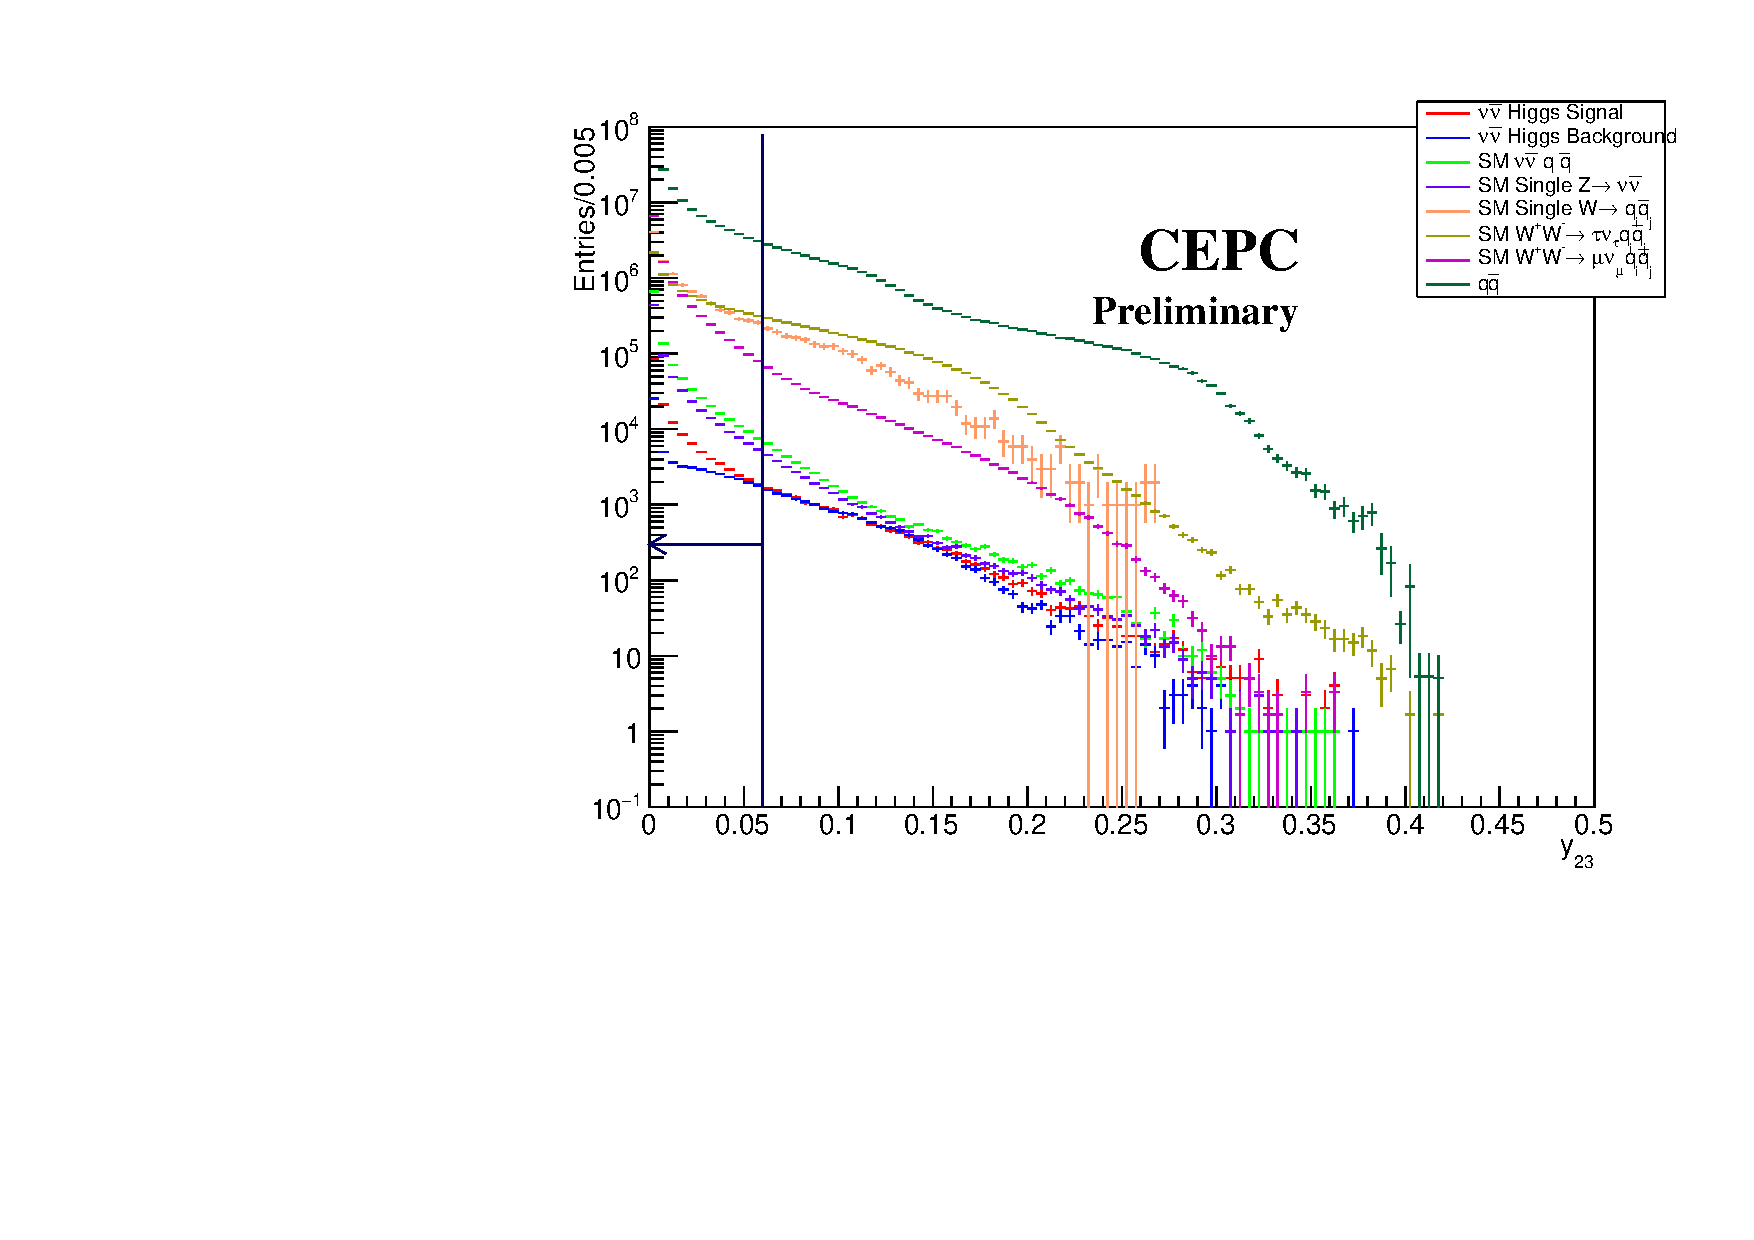
\includegraphics[width=\textwidth]{Analysis/nnh/y23.pdf}
  \end{minipage}
}
\subfigure[]
{
  \begin{minipage}[b]{0.31\textwidth}
  \includegraphics[width=\textwidth]{Analysis/nnh/y34.pdf}
  \end{minipage}
}
\caption{The $y_{12}$(left), $y_{23}$(middle) and $y_{34}$ right distribution in \nnh analysis.}
\end{figure}

\begin{figure}[!htbp]
\label{fig:BDT_nnh}
\centering
\subfigure[]
{
  \begin{minipage}[b]{0.42\textwidth}
  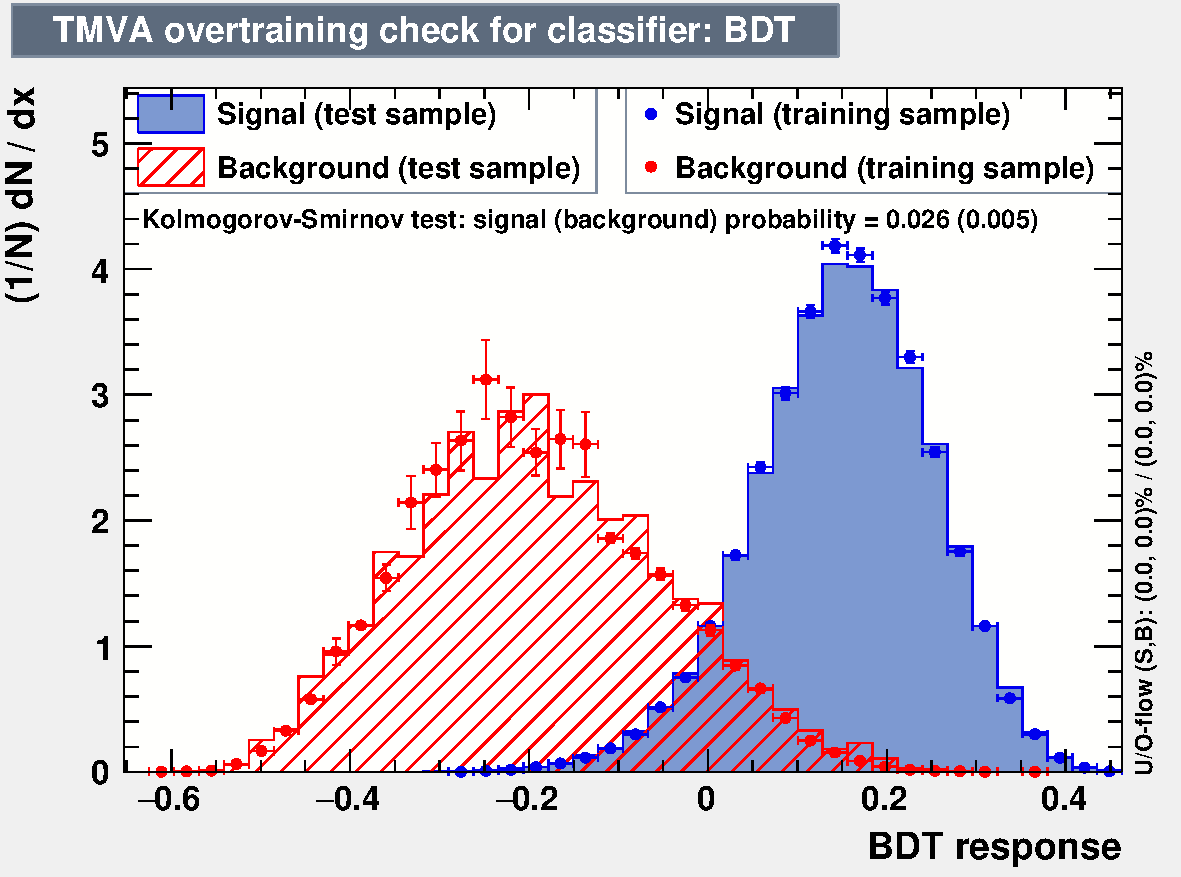
\includegraphics[width=\textwidth]{Analysis/nnh/overtrain_BDT.pdf}
  \end{minipage}   
}
\subfigure[]
{
  \begin{minipage}[b]{0.42\textwidth}
  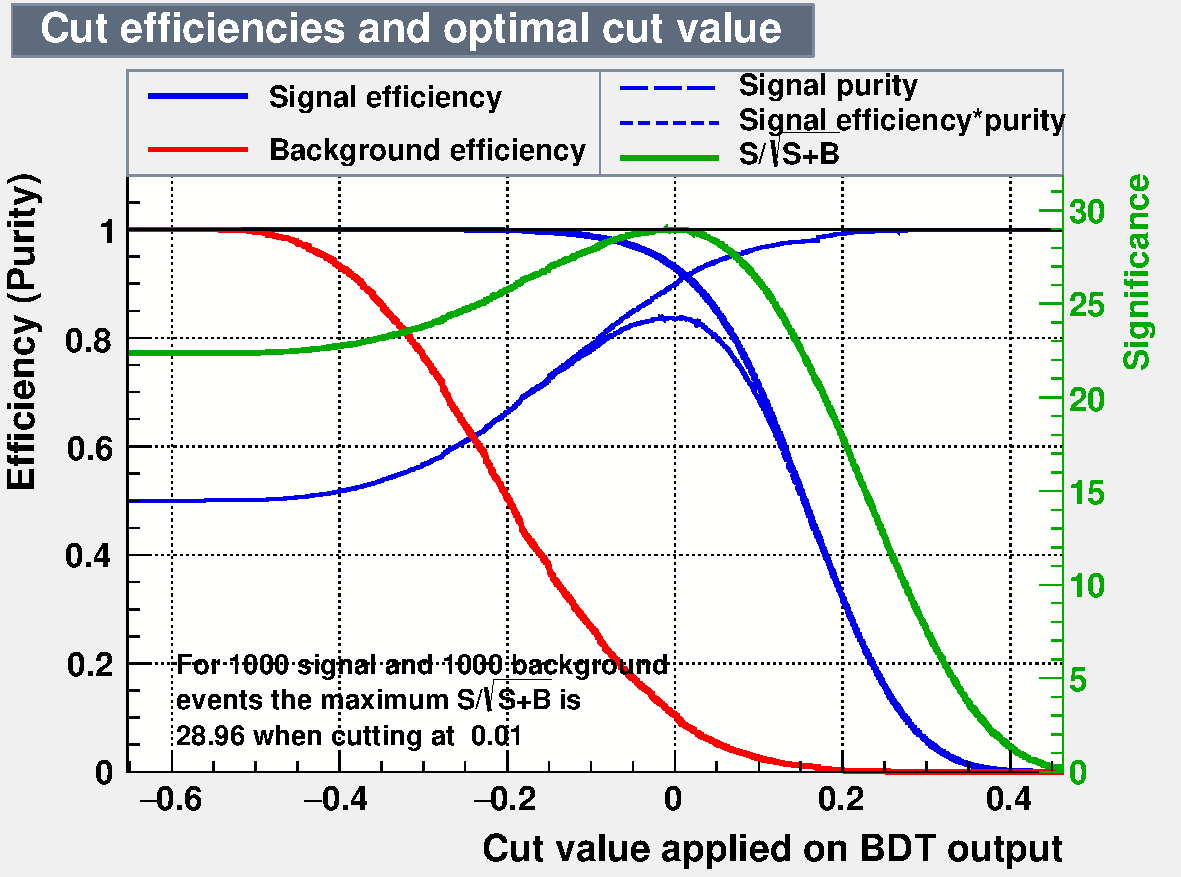
\includegraphics[width=\textwidth]{Analysis/nnh/mvaeffs_BDT.pdf}
  \end{minipage}
}
\caption{Over training check of BDT distribution(left) and optimization of the 
BDT cut performance.}
\end{figure}

\begin{table}[!htbp]
\chuhao
\label{tab:nnh_cut}
\center
\begin{tabular}{c|c|c|c|c|c|c|c|c}\hline
cutflow                 &signal          &\nnh bkg          &zzsl             &sznuqq          &wwsltauq         &wwslmuq           &swslqq           &qq                \\ \hline 
No Cut                  &170633          &76604.1         &\ten{1.08992}{6} &744218          &\ten{1.19114}{7} &\ten{1.19114}{7}  &\ten{1.30255}{7} &\ten{2.46847}{8}  \\ \hline 
2 jets in final state   &170512          &73227.4         &\ten{1.08987}{6} &744201          &\ten{1.19112}{7} &\ten{1.19112}{7}  &\ten{1.30255}{7} &\ten{2.46842}{8}  \\ \hline 
NPFO                    &170349          &42734.8         &980878           &656657          &\ten{1.17604}{7} &\ten{1.16597}{7}  &\ten{1.22262}{7} &\ten{2.39672}{8}  \\ \hline 
$E_{total}$             &152374          &33867.2         &451233           &250618          &\ten{5.06253}{6} &\ten{1.27372}{6}  &\ten{2.07027}{6} &\ten{1.01743}{8}  \\ \hline 
pT                      &142048          &31579.8         &413994           &229568          &\ten{4.31686}{6} &\ten{1.19619}{6}  &\ten{1.93607}{6} &297012            \\ \hline 
IsoLep Veto             &141112          &27966           &410719           &227762          &\ten{3.73815}{6} &365116            &682854           &294929            \\ \hline 
$M_{inv}$               &134583          &26165.2         &41340.5          &23255.3         &\ten{2.20577}{6} &66320             &336493           &111687            \\ \hline 
$M_{recoil}$            &125958          &24817.4         &37889.9          &20720.1         &\ten{1.75479}{6} &29908             &237815           &85653.4           \\ \hline 
y12                     &125228          &24164.8         &37138.4          &20306.8         &\ten{1.61702}{6} &27807.4           &228934           &83451.1           \\ \hline 
y23                     &126365          &13478.1         &29136.3          &15976.7         &\ten{1.07172}{6} &18577.8           &126308           &71353             \\ \hline 
y34                     &107347          &5708.84         &26728            &14616.3         &889531           &16016             &110520           &69372.9           \\ \hline 
costheta                &104023          &5169.31         &21169.6          &11891.4         &506063           &9354.92           &85850.1          &48209.6           \\ \hline 
BDT Cut                 &83852.1         &1961.65         &2704.18          &1566.07         &11116.3          &476.269           &986.783          &6170.45           \\ \hline         
\end{tabular}
\caption{Signal and background yields in the cutflow of \nnh analysis, normalized to 5000 \ifb}
\end{table}

%\clearpage




\subsection{$\qqh$ Event Seleciton} 
The $\qqh$ channel refers to $ZH$ production in which both $Z$ and Higgs bosons decays hadronically.
We require exclusively 4 jets reconstructed by Durham-like algorithm\cite{Durham} in final states, corresponding to the leading logrithm approximation of 4-partners final states. The domiant SM backgrounds are consist of diboson production followed by hadronic decays of both bosons, and quark pair production. Events with loosened isolation lepton candidates were rejected.
All of the 4 jets are required to contain at least 10 PFOs to remove the 
events with fake jets. 
The visible energy of each event are required to be larger than 206 \GeV 
to reject the events with energetic nuetrinos. 
In figure \ref{fig:VisEn_nPFO} visible energy and minimum PFO multicplicity of the jets distributions of signal and backgrounds are presented.\par
\begin{figure}
\label{fig:VisEn_nPFO}
\centering
\subfigure[]
{
  \begin{minipage}[b]{0.42\textwidth}
  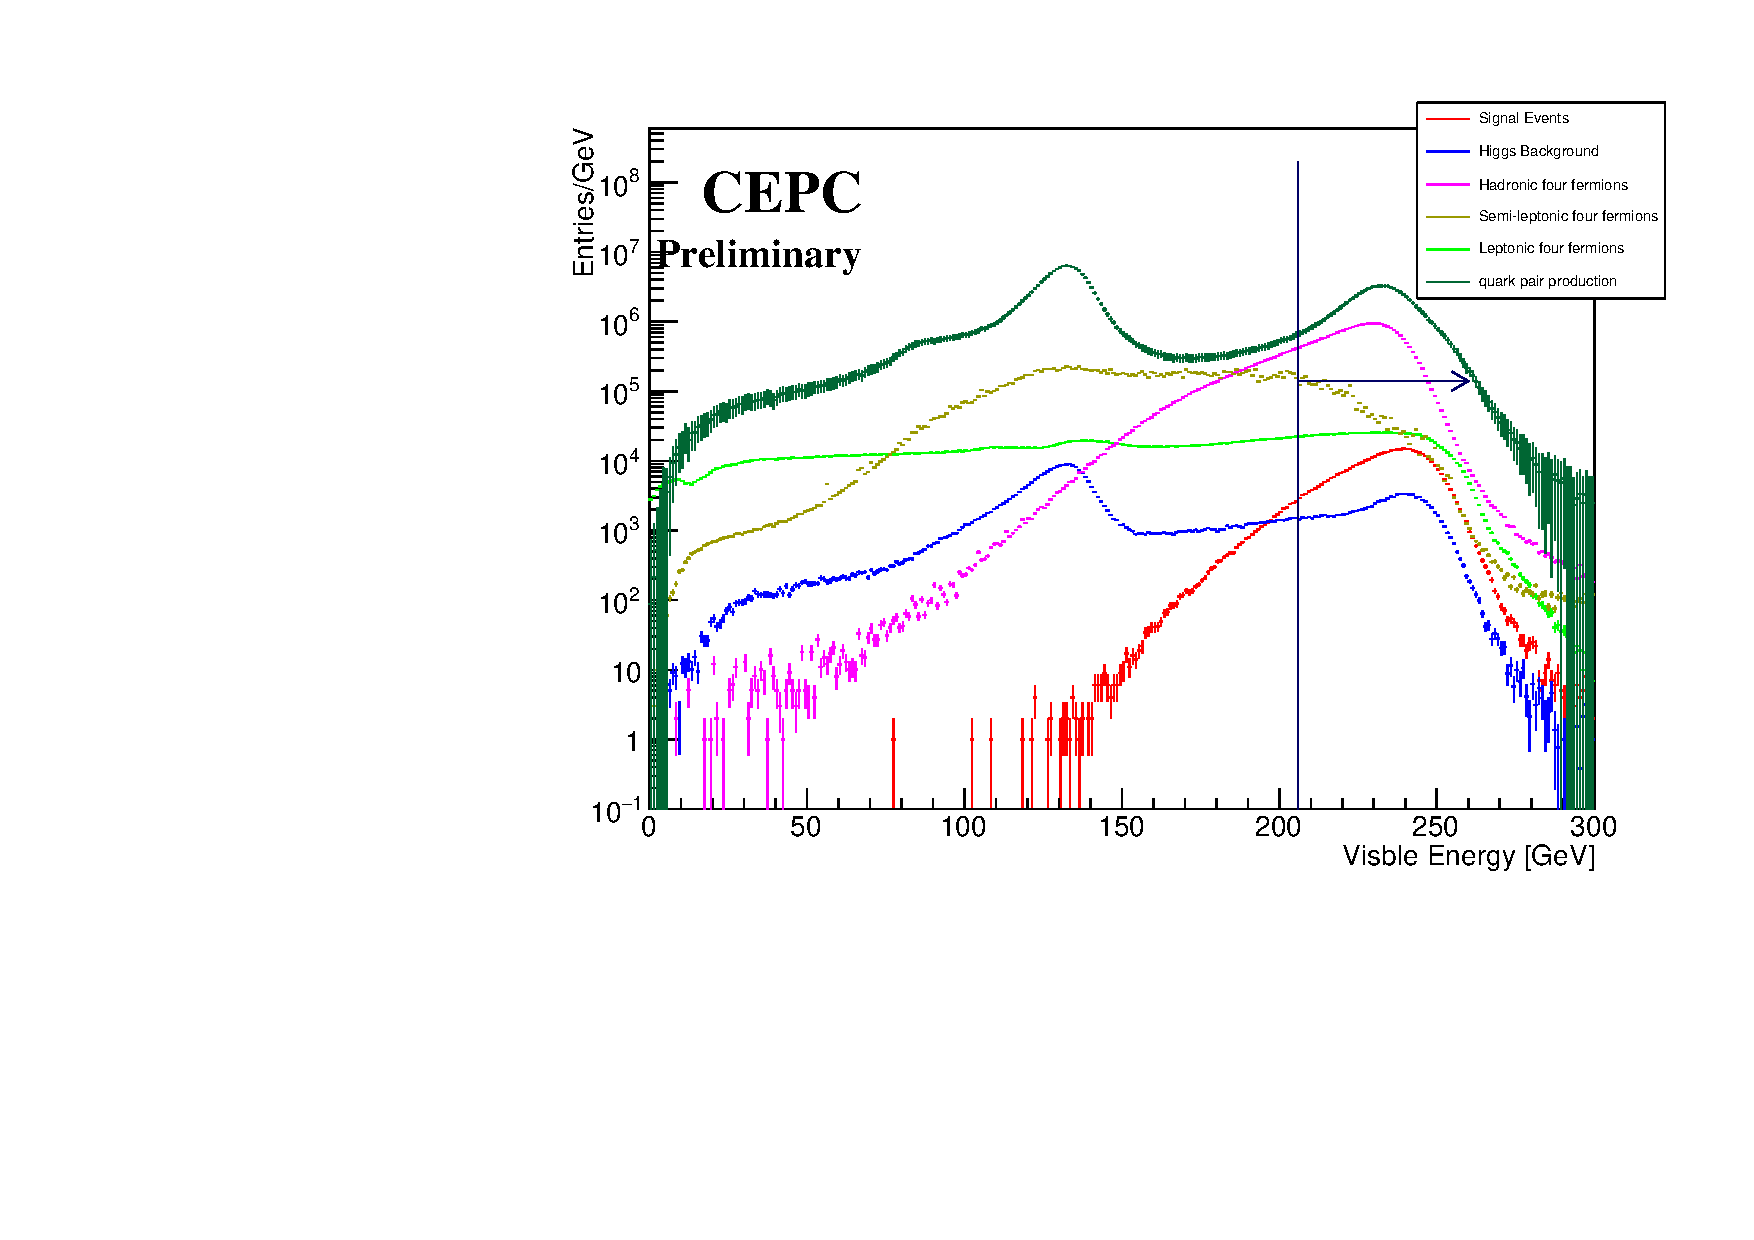
\includegraphics[width=\textwidth]{Analysis/qqh/VisEn.pdf}
  \end{minipage}
}
\subfigure[]
{
  \begin{minipage}[b]{0.42\textwidth}
  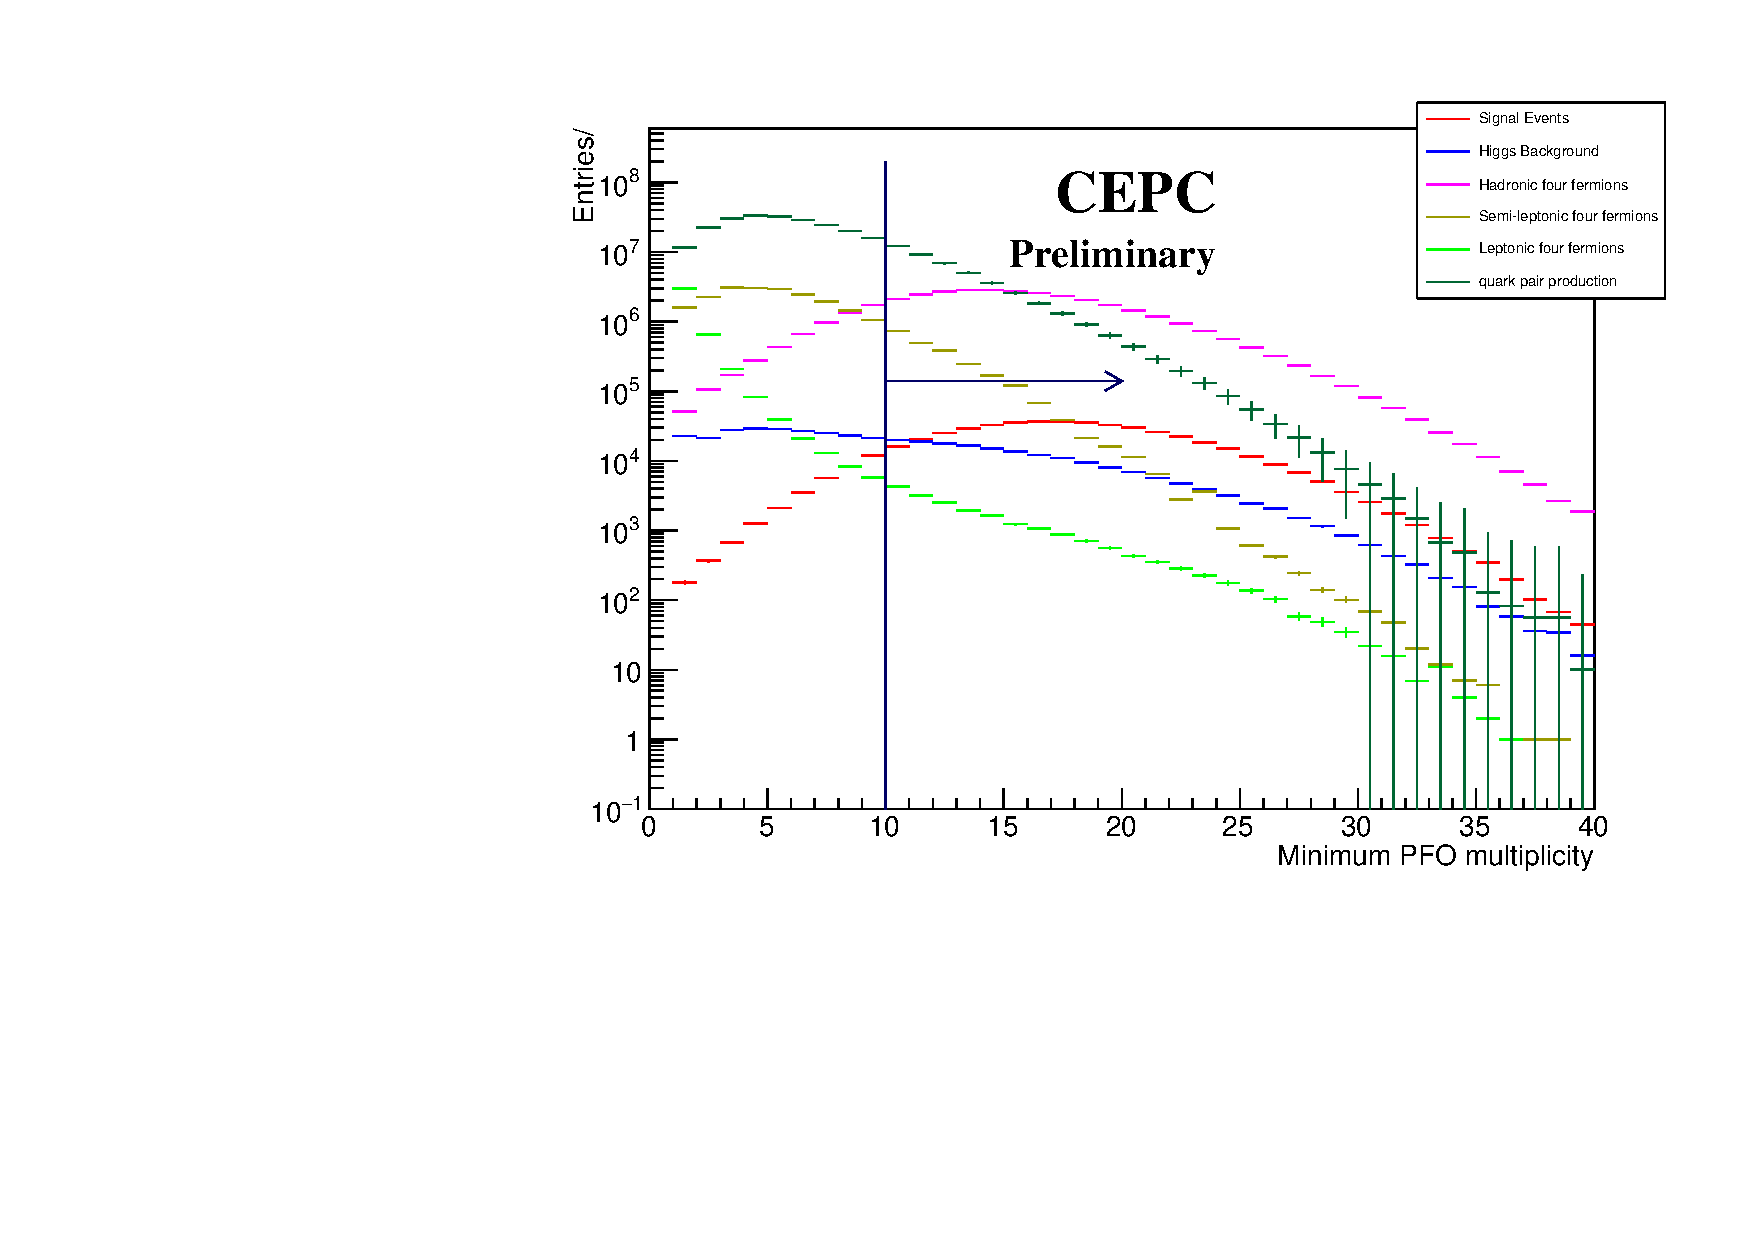
\includegraphics[width=\textwidth]{Analysis/qqh/nPFOmin.pdf}
  \end{minipage}
}
\caption{Distribution of visible energy(left) and minimum jets' pfo multiplicity(right) for the signal and SM backgrounds.}
\end{figure}


%It can also effectively remove the 2 fermions events with radiation return, since emitted photon can be missed from detection.

%To further suppress the background from 2 jets events, two variable are used as discriminator. One is called yth-value('th' refer to 3 and 4 here) which is constructed from PFO distributionthe other one is called sphericity, which represents the PFO distribution shape in each event. The distribution of \emiss, $y_34$ and sphericity can be found in figure \ref{fig:missingE}.
To suppress the background from 2 jets events, the $y_{34}$ are used as discriminator, which can effectively select the 4 jets events 
from those with lower jet multiplicity. A cut on the energetic-weighted angular 
dispersion was defined as $\Delta\theta$ variable, 
which was used in ALEPH 4-bjets channel analysis\cite{ALEPH_ZH_PLB}, is also used to furuther suppress the $q\bar{q}$ and semi-leptonic 4 fermions backgrounds.
 . The distribution of $y_{34}$ and $\Delta\theta$ can be found in figure 
 \ref{fig:y34_Deltatheta}.
 \begin{figure}
\label{fig:y34_Deltatheta}
\centering
\subfigure[]
{
  \begin{minipage}[b]{0.42\textwidth}
  \includegraphics[width=\textwidth]{Analysis/qqh/y34.pdf}
  \end{minipage}
}
\subfigure[]
{
  \begin{minipage}[b]{0.42\textwidth}
  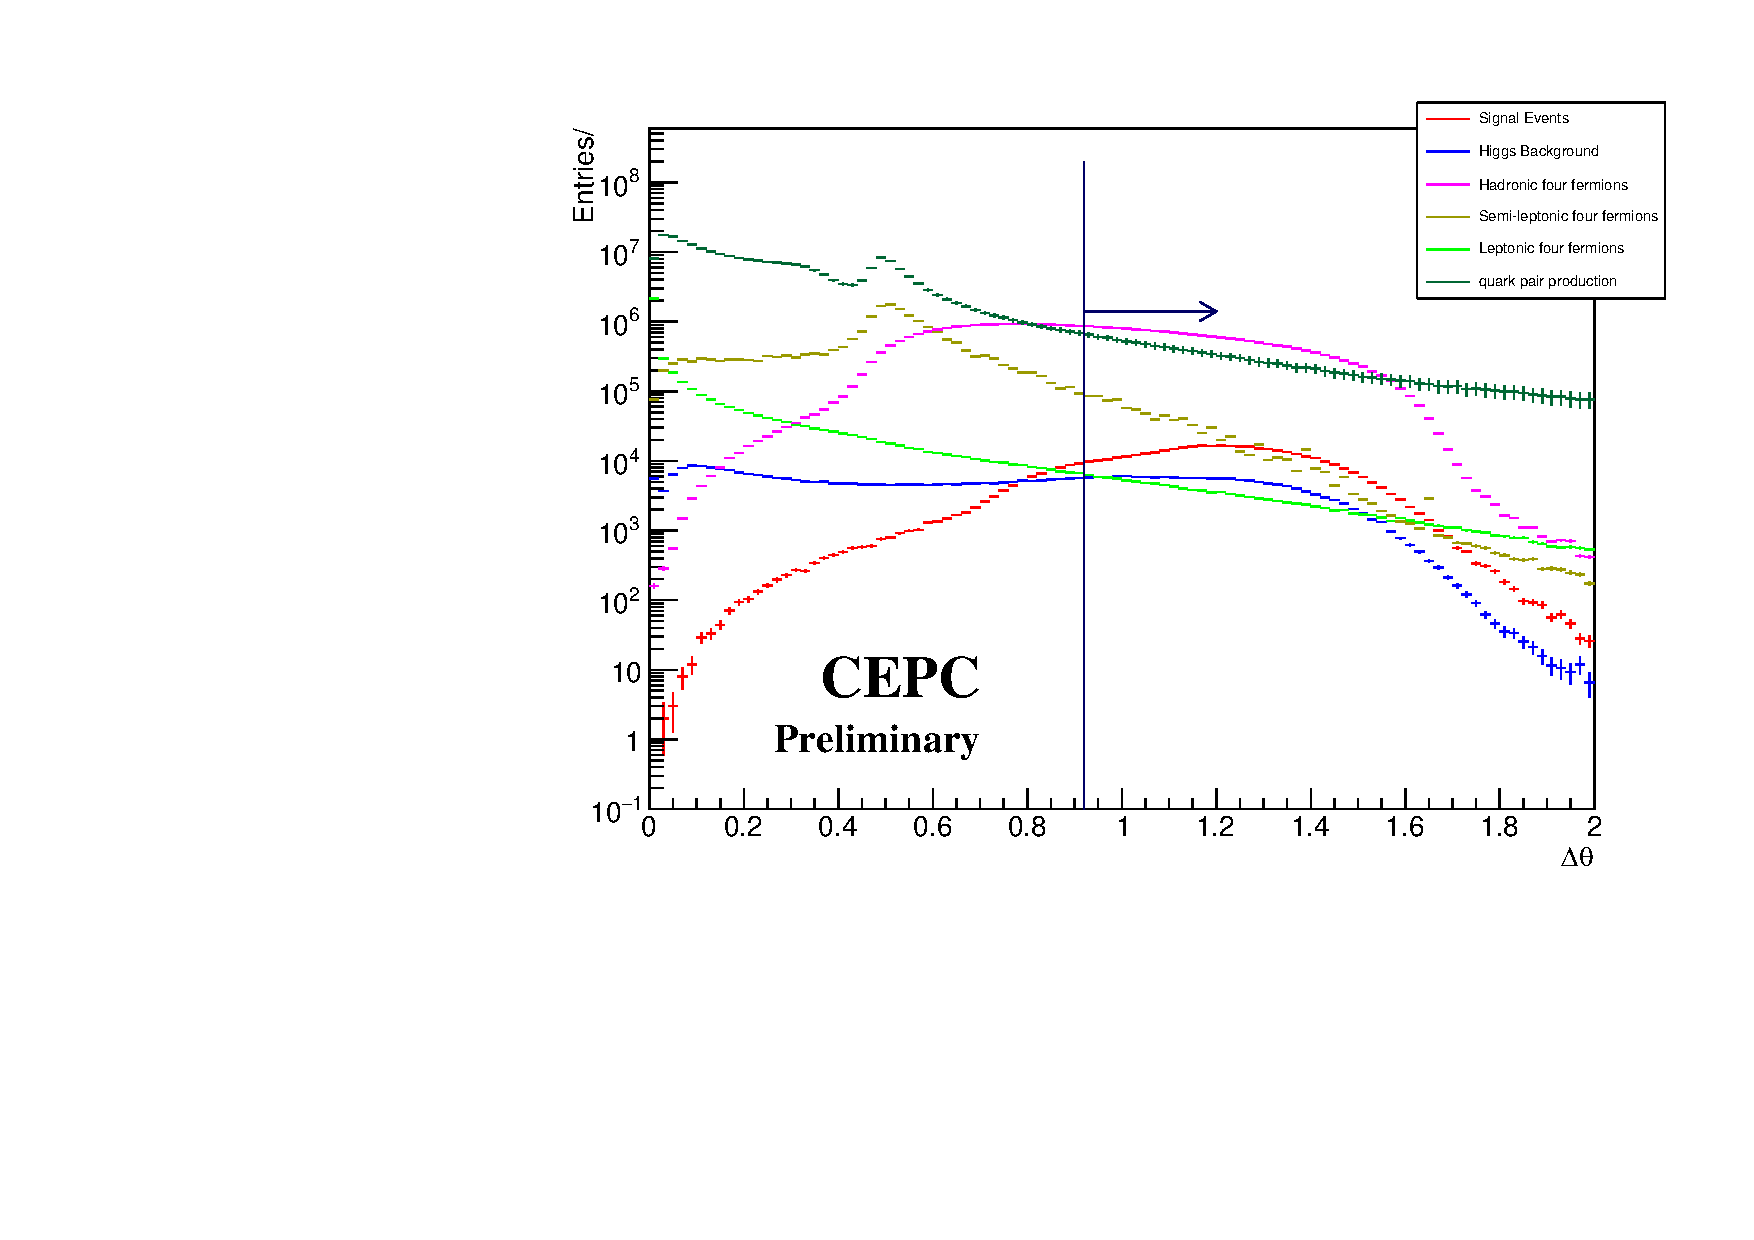
\includegraphics[width=\textwidth]{Analysis/qqh/DeltaTheta.pdf}
  \end{minipage}
}
\caption{Distribution of $y_{34}$(left) and $\Delta\theta$ (right) for the signal and SM backgrounds.}
\end{figure}
 \par 
%\begin{figure}[htpb]
%\centering
%    \includegraphics[width=0.45\textwidth]{figures/MissingE.pdf}
%    \includegraphics[width=0.45\textwidth]{figures/y34.pdf}
%    \includegraphics[width=0.45\textwidth]{figures/Sphericity.pdf}
%\caption{Distribution of MissingE, $y_{34}$ and sphericity of signal and background events, normalized to 5000 fb$^{-1}$
%}
%\label{fig:missingE}
%\end{figure}

The 4 jets in the final states are paired in order to get minimum $\chi^2$ defined as:
\begin{equation}
     \chi^2_{HZ} = \mathrm{min}\{(m_{ij}-m_H)/\sigma^2_{H} + (m_{kl}-m_Z)/\sigma^2_{Z} \}
     \label{for:chi2}
\end{equation}
in which i,j,k,l are the jet index, running from 1-4; $m_{ij}$ is the invariant mass of one jet pair and $m_{kl}$ is that of another pair; $m_H$ and $m_Z$ are Higgs and Z boson mass; $\sigma_H$ and $\sigma_Z$ are the width of reconstructed jet pair invariant mass from Higgs and  $Z$ boson. A variable $\chi^2_{WW}$ is defined in the similar way as formula \ref{for:chi2}, in which the $Z$/Higgs masses and widths are replaced by those of $W$ boson. The $\chi^2_{HZ}$ and $\chi^2_{ZZ}$ are combined into a variable $X$:
\begin{equation}
  X = \dfrac{\chi^2_{WW}-\chi^2_{HZ}}{chi^2_{WW}+\chi^2_{HZ}}
  \label{for:X}
\end{equation}
 The X value distrutes in the range from -1 to 1. For signal events, it tends to be positive 
 values(close to 1) while for the dominant $WW$ hadronic background, the X value tends to be negative(close to -1), as shown in figure \ref{fig:X}. Thus X provides discrimination power against $WW$ hadronic events.
 \begin{figure}
 \label{fig:X}
 \centering
 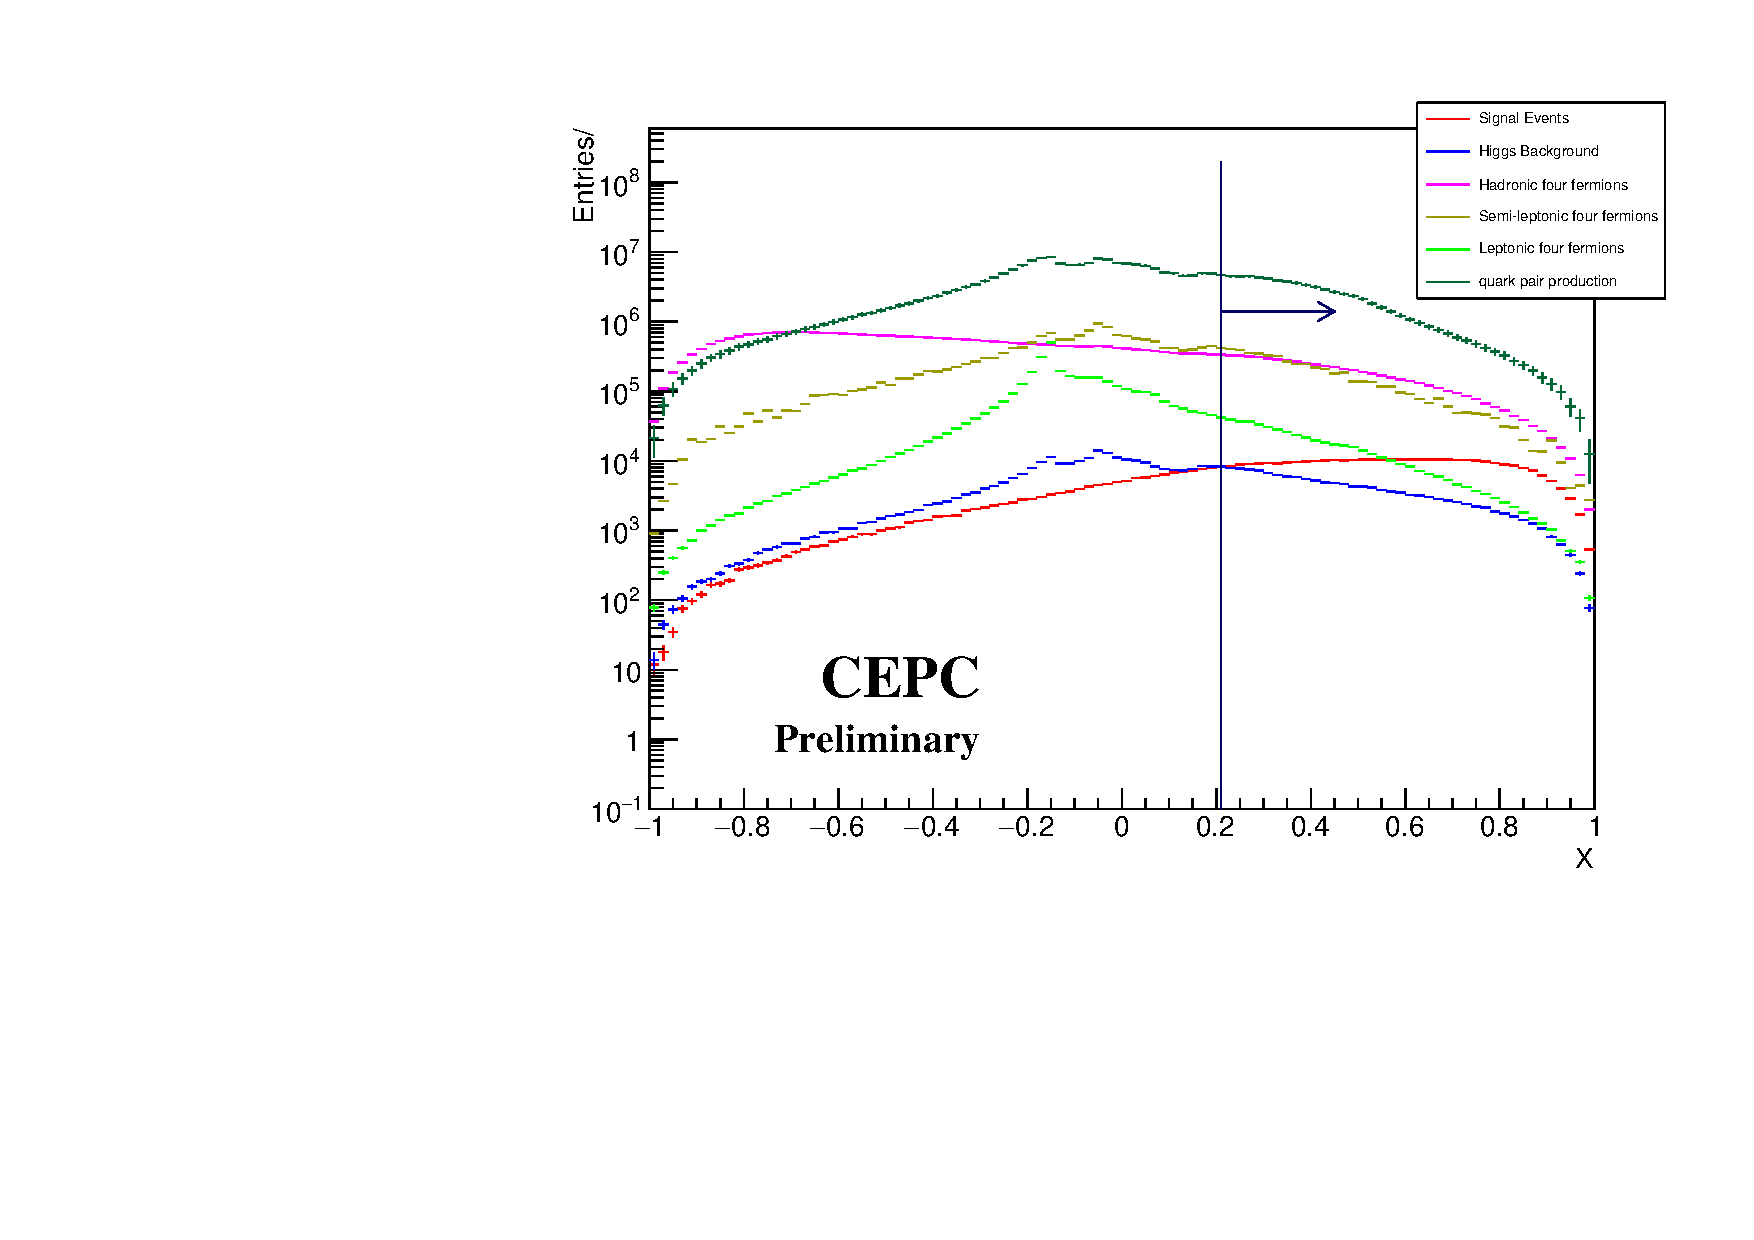
\includegraphics[width=0.67\textwidth]{Analysis/qqh/X.pdf}
 \caption{The distribution of $X$ defined in formula \ref{for:X}.}
 \end{figure}
\par
%invariant mass distribution of 2 jets from Higgs or Z correspondingly.  The distribution of 2 jet pair invariant mass can be found in figure \ref{fig:jet_pair_invmass}
%\begin{figure}[htpb]
%\centering
%    \includegraphics[width=0.45\textwidth]{figures/HZ_signal.eps}
%    \includegraphics[width=0.45\textwidth]{figures/HZ_4q.eps}
%\caption{Distribution of invariant mass of the two jet pairs for signal(left) and WW(right) events. The x-axis represents the invariant mass of a jet pair which is cloest to the higgs among all combination; the y-axis represents the invariant mass of another jet pair.
%}
%\label{fig:jet_pair_invmass}
%\end{figure}

%The results of the cutflow are summerized in table \ref{tab:cutflow}.
%\begin{table}[!htbp]
%\centering
%\begin{tabular}{|c|c|c|c|c|c|c|c|c|c|} \hline
%         &   signal   & other qqH      &  ffH   &  qq   &  ll   &  qqqq  &   llqq   &  lvqq   & vvqq  leptonic \\ \hline
%Dataset  &  \multicolumn{2}{c|}{724k}  &  405k  & 250M  & 20.4M & 36.9M  &  3.2M    &  36.45M &  2.17M    \\ \hline
%  4J FS  &  494.6k    &   214.2k       & 299.4k &\multicolumn{2}{c|}{267.1M}
%                                                                & 36.85M &  3.16M   &  35.9 M & 1.36M   \\ \hline
%  Iso Lep Veto
%         & 489.7k     &   154.4k       & 130.9k &\multicolumn{2}{c|}{242.2M}
%                                                                & 36.2M  & 558.4k   &  9.33M  & 1.35M     
%                                                                \\ \hline
%  \emiss$<$76 GeV
%         & 487.3k     &   130.2k       & 15.9k  &\multicolumn{2}{c|}{238.8M}
%                                                                & 36.11M & 354.5k   &  3.1M   & 964         \\ \hline
%  $y_{34}>$0.013
%        & 339.1k     &  99.34k        & 8.71k  &\multicolumn{2}{c|}{12.58M}
%                                                                & 20.83M & 78.25k   & 345.2k  & 88      \\ \hline
%  sphericity$>$0.44
%        & 315.1k     &  92.8k         & 7.87k  &\multicolumn{2}{c|}{2.88M}
%                                                                & 16.84M & 56.1k    & 194.5k  & 34    \\   \hline
%  Min($\chi^2 <$18) 
%        & 240.7k     & 61.7k         & 2.6k   &\multicolumn{2}{c|}{1.69M}
%                                                                & 10.1M  & 15.96k   & 13.52k  &  0   \\ \hline                                                  
%                                                                            
%     
%\end{tabular}
%\caption{ Event yields of signal and background in cutflow, normalized to 5000 fb$^{-1}$} 
%\label{tab:cutflow}
%\end{table}
The BDT\cite{BDT} method is applied to further suppress the SM backgrounds. The variables like 
reconstructed Higgs and $Z$ mass, different combination of jet pair invariant masses, $y_{34}$ 
and $y_{45}$ and sphericity, reconstructed $Z$ and Higss $\cos \theta$ and highest energy of 
of jets are used in the training. Figure \ref{fig:qqh_BDT} shows the signal and background distribution of linear correlation of these variables and the outcome BDT response of signal and backgrounds.
\begin{figure}
\label{fig:qqh_BDT}
\centering
\subfigure[]
{
  \begin{minipage}[b]{0.42\textwidth}
  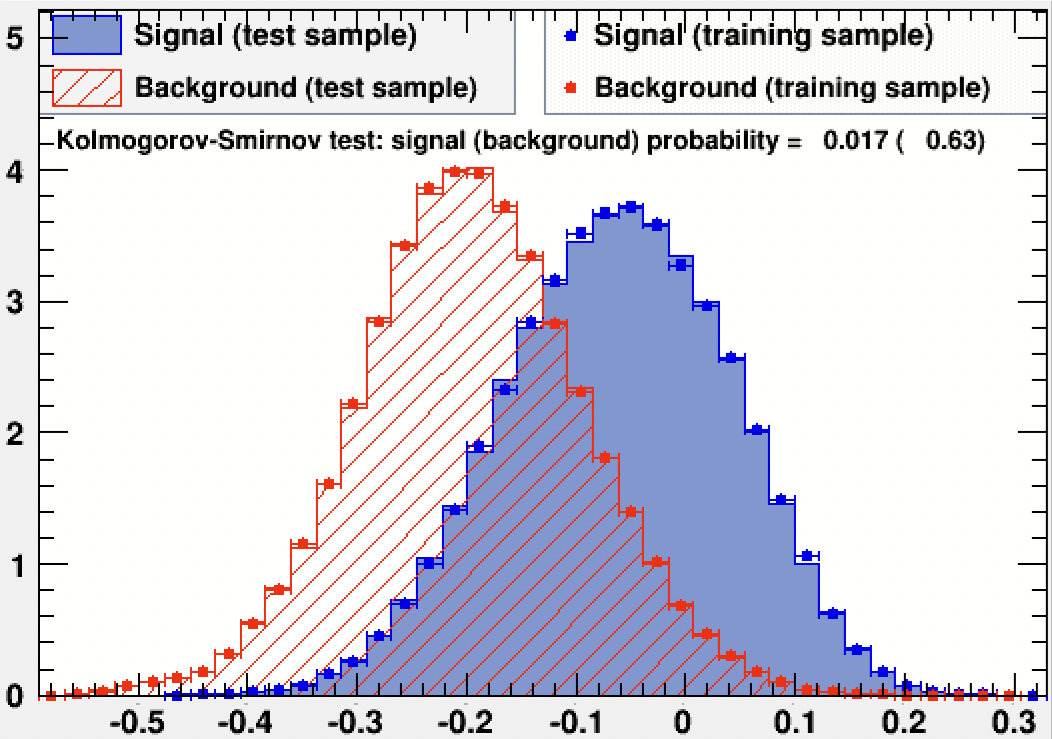
\includegraphics[width=\textwidth]{Analysis/qqh/BDT.png}
  \end{minipage}
}
\subfigure[]
{
  \begin{minipage}[b]{0.42\textwidth}
  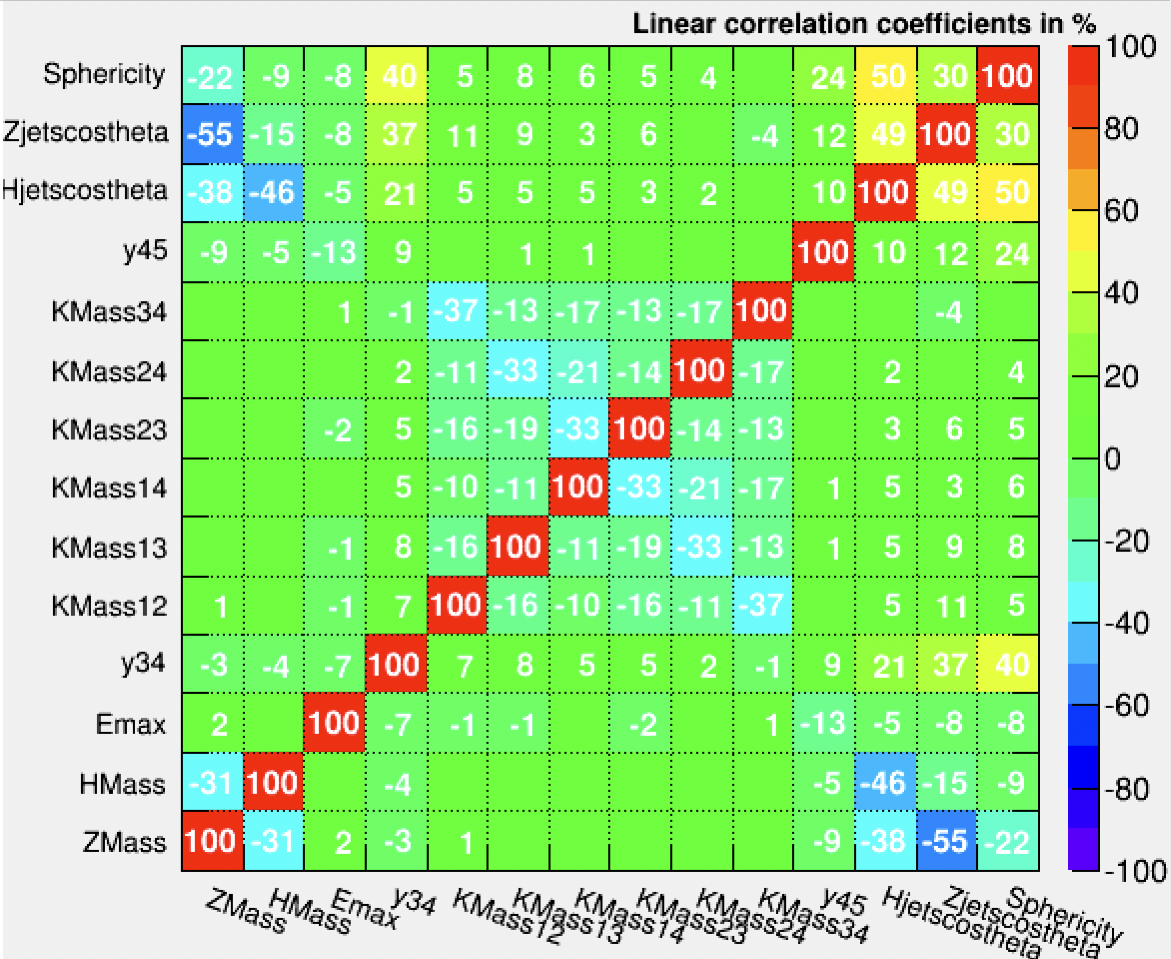
\includegraphics[width=\textwidth]{Analysis/qqh/Correlation.png}
  \end{minipage}
}
\caption{Linear correlation map of variables used in BDT training(left) and the outcome BDT 
response of signal and backgrounds.}
\end{figure}


\begin{table}[!htpb]
\centering
\chuhao
\begin{tabular}{c|c|c|c|c|c|c|c|c|c}\hline
         & \tabincell{c}{signal \\ combined}   &  $\Hboson \to \bpair$   & $\Hboson\to\cpair$   & $\Hboson\to\gpair$   & \tabincell{c}{background\\ combined} & \tabincell{c}{higgs \\background}   &   \tabincell{c}{4 fermions\\ hadronic}&  quark pair &  \tabincell{c}{4 fermion\\ semi-leptonic}  \\ \hline 
 4 jets and iso-lepton veto 
         &  493947 & 413299   & 19362  & 61286  &     75 M      &  299583  &  36.83 M &   23.86M   &   14.72 M      \\ \hline
  $E_{vis} > $206 GeV
         &  459972 &  381470  & 18690  & 59812  &     50.6 M    &  109529  &  28.19 M  &  20.37M  &  1.967M  \\ \hline
 $y_{34} > 0.007$
         &  393979 &  325137 &   15976  & 52866 & 26.4 M        &   100813 &  21.32 M  &  5.207 M  &  218394 \\ \hline
 $N_{jet,pfo} \ge 9$
         &  371240 &  305982 &   14903  & 50355 & 21.4 M        &    82281 &  18.78 M  & 
2.601 M  &  27487  \\ \hline
 $\Delta \theta > $0.92
         &  318163 &  261808 &   12610  & 43745 & 13.55 M       &    71987 &  12.16 M &  
1.315 M  &  4745   \\ \hline
   $X > 0.21$
         &  236652 &  197510 &    9562  & 29580 & 3.15 M        &    38579 &  2.2 M   &  907188   &  3012   \\ \hline
   $BDT > $-0.19
         &  211281 &  177447 &    8324  & 25510 & 1.52 M        &    32653 &  1.08 M  & 
405567   &  580    \\ \hline   
      
\end{tabular}
\caption{Signal and background yields of cutflow in \qqh analysis, normalized to 5000 \ifb}
\label{tab:cut_qqh}
\end{table}


A yth-value is defined according to the PFOs distribution to suppress the background from di-jet events. 
